%\documentclass{report}
\documentclass[11pt,letter,notitlepage]{article}
\usepackage[margin=1in]{geometry}
\usepackage{setspace}
\usepackage{times}
\title{
	\textsc{ \small
		Washington State University \\
		School of Electrical Engineering and Computer Science \\
		EE 352, Electrical Engineering Laboratory
	} \\
	{\textsc{\small Lab Project}} \\
	AM Transmitter/Receiver
}

\author{Kevin Evans \\
\small{Partners: Jacob Hnatiak, Aman Amad al-Ameedi}}
\date{May 1, 2020}

% start sections at 1 with subsections to 1.1, 1.2...
\renewcommand{\thesection}{\arabic{section}}

%alias for vpp/rms
\newcommand{\pp}{_{pp}}
\newcommand{\rms}{_{rms}}
\newcommand{\Vpp}{\V\pp}
\newcommand{\Vrms}{\V\rms}

\usepackage{siunitx}
\usepackage{threeparttable}
\usepackage{booktabs}
\usepackage{multirow}
\usepackage{graphicx}
\usepackage{float}
\usepackage{amssymb,amsmath}
\usepackage{physics,cancel}
\usepackage{listings}
\usepackage{steinmetz} % \phase{}
\usepackage{mathtools} % for '\mathclap' macro
\usepackage{caption,subcaption} %multiline captions; subfigures


% for MATLAB code
\usepackage{courier}
\renewcommand{\lstlistingname}{Code Snippet}

\lstset{basicstyle=\footnotesize\ttfamily,breaklines=true}
%\lstset{framextopmargin=50pt,frame=bottomline}
\lstset{language=Matlab,%
	%basicstyle=\color{red},
	breaklines=true,%
	morekeywords={matlab2tikz},
	keywordstyle=\color{blue},%
	morekeywords=[2]{1}, keywordstyle=[2]{\color{black}},
	identifierstyle=\color{black},%
	stringstyle=\color{mylilas},
	commentstyle=\color{mygreen},%
	showstringspaces=false,%without this there will be a symbol in the places where there is a space
	%	numbers=left,%
	%	numberstyle={\tiny \color{black}},% size of the numbers
	%	numbersep=9pt, % this defines how far the numbers are from the text
	emph=[1]{for,end,break},emphstyle=[1]\color{red}, %some words to emphasise
	emph=[2]{zpkdata, tf}, emphstyle=[2]{\color{blue}},    
}
\usepackage{pdflscape}

\usepackage{color} %red, green, blue, yellow, cyan, magenta, black, white
\definecolor{mygreen}{RGB}{28,172,0} % color values Red, Green, Blue
\definecolor{mylilas}{RGB}{170,55,241}

\usepackage[hidelinks]{hyperref}

\begin{document}
	
	\maketitle
	\begin{abstract}
		\noindent In this project, an AM transmitter and receiver was designed and simulated using LTspice. The AM transmitter uses an input message signal between \SI{400}{\Hz} and \SI{8}{\kHz} and mixes the signal with a carrier frequency of \SI{72}{\kHz}, generated by a Wien oscillator. The transmitter amplifies the signal to be carried across a \SI{50}{\ohm} BNC cable to the receiver with \SI{50}{\ohm} impedance. The receiver uses a peak detector with a Butterworth bandpass filter to detect and restore the envelope message signal. This signal is passed to a Schmitt trigger comparator and a buffer amplifier, which drives an \SI{8}{\ohm} speaker. The project was simulated using LTspice. The simulations show that the transmitter-receiver design met the required specifications.
	\end{abstract}

	\clearpage
	\section{Introduction}
	In this project, a transmitter was designed to transmit an amplitude modulated (AM) signal across a BNC cable and a receiver will restore the original message signal and output the signal through a speaker. In amplitude modulation, a carrier signal is used to transmit a message signal. This is done by modulating the carrier amplitude proportionally to the message signal, as depicted in Figure \ref{fig:am}. This idea is particularly useful when transmitting over-the-air, as the receiver must only know the transmission frequency and a bandwidth to receive a message signal. 
	
	\begin{figure}[h]
		\centering
		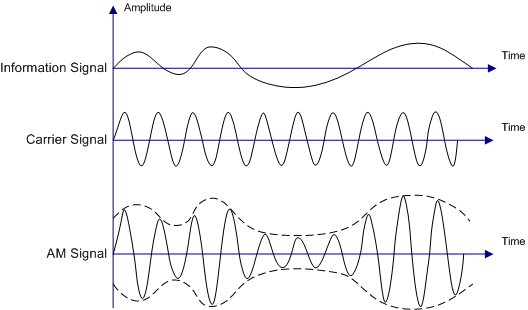
\includegraphics[width=0.7\linewidth]{am}
		\caption{The basic principle of amplitude modulation (AM)\protect\footnotemark.}
		\label{fig:am}
	\end{figure}	
	\footnotetext{{Image is adapted from \textit{Illustration of Amplitude Modulation}, Ivan Akira. \newline
	 {\hspace*{1.5em} \url{https://commons.wikimedia.org/wiki/File:Illustration\_of\_Amplitude\_Modulation.png}}}}
	
	The outline of the project is depicted in the block diagram in Figure \ref{fig:radiodiagram}. First, the input message signal will be mixed with the carrier oscillator signal, generated by a Wien oscillator. A switching modulator will mix the signals by proportionally adding the two signals, relative to a modulation index. Next, a high quality bandpass filter will be used to filter the half-wave output of the modulator, allowing only a narrow band of signals allowed near the carrier frequency. A power amplifier is then employed to buffer the signal and to increase the current driven across the transmission line, a BNC cable.
	
	After transmission through a BNC cable, a combination of a peak detector and a Butterworth bandpass filter will detect and restore the envelope message signal. A comparator using a Schmitt trigger and a diode is used to convert the sinusoid signal into a pulsed waveform. From these pulse waves, a buffer amplifier can drive a speaker to product audible sounds. Verification of meeting the specifications will come through time- and frequency-domain simulations done through LTspice. The output waveforms of each component is captured through the simulations and will be analyzed to determine if the specifications are met.
	\clearpage
	
	\subsection{Specifications}
	For the project, the following requirements must be met:
	\begin{enumerate}
		\item Components are limited to those in the analog parts kit.
		\item Power supplies: $\pm$ \SI{12}{\V} DC.
		\item Input: Single tone sine wave from a bench generator; frequencies \SI{500}{\Hz} to \SI{4}{\kHz}.
		\item Output: Single tone sine wave, displayed on an oscilloscope and played through a speaker.
		\item Carrier frequency: between \SI{60}{\kHz} and \SI{80}{\kHz}.
		\item Transmitter bandpass filter specifications: \begin{enumerate}
			\item Lower stop band: $\abs{H(j \omega)} \le \SI{-20}{\dB}$ for frequencies $f < \SI{4}{\kHz}$.
			\item Upper stop band: $\abs{H(j \omega)} \le \SI{-210}{\dB}$ for frequencies twice the carrier frequency, $f = 2 f_c$.
			\item Pass band: $\SI{-1}{\dB} \le \abs{H(j \omega)} \le \SI{1}{\dB}$ for frequencies between $f = f_c \pm \SI{4}{\kHz}$.
		\end{enumerate}
	\end{enumerate}
	\clearpage
	
	\begin{landscape}
		\subsection{Block diagram}
		\begin{figure}[h]
			\centering
			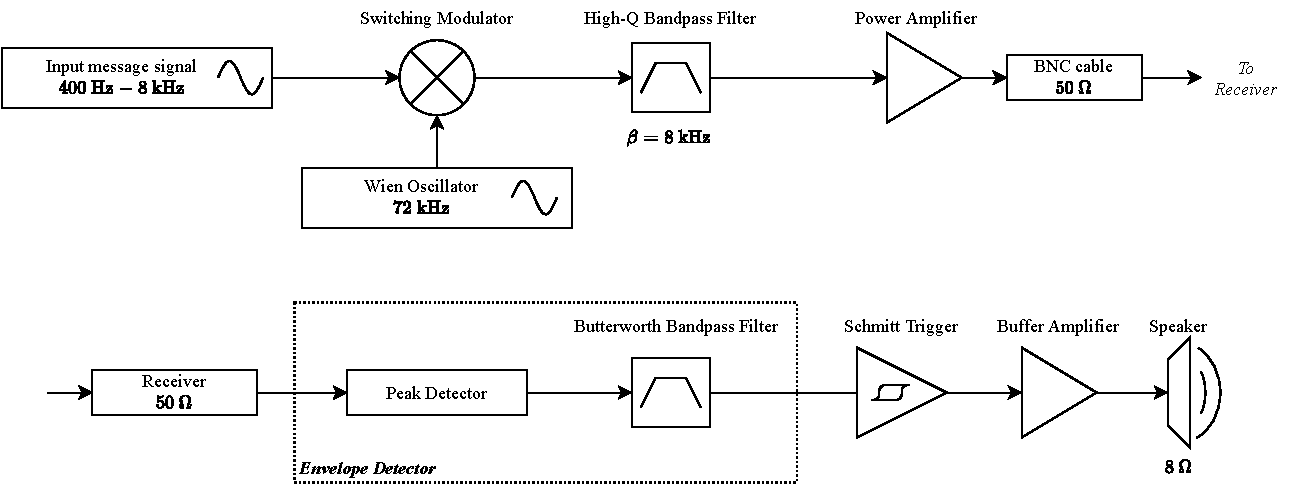
\includegraphics[width=\linewidth]{radiodiagram}
			\caption{A block diagram of the components used in this AM radio.}
			\label{fig:radiodiagram}
		\end{figure}
	\end{landscape}
	\clearpage %%%%%%%%%%%%%%%%%%%%%%%%%%%%%%%%%%%%%%%%%%%%%%%%%%%
	\section{Design and Simulation Results}
	\subsection{Wien bridge oscillator}
	The Wien bridge oscillator is a sinusoidal oscillator utilized in the circuit to produce the carrier signal. The basic design of this oscillator uses an op-amp and an RC network. The RC network selects a target frequency and loops back into the non-inverting input of amplifier. Over a short period of time, the oscillator stabilizes around the target frequency with little drift. The oscillator circuit is shown below in Figure \ref{fig:wienckt} with the its RC networks highlighted, $Z_s$ and $Z_p$.
	
	\begin{figure}[h]
		\centering
		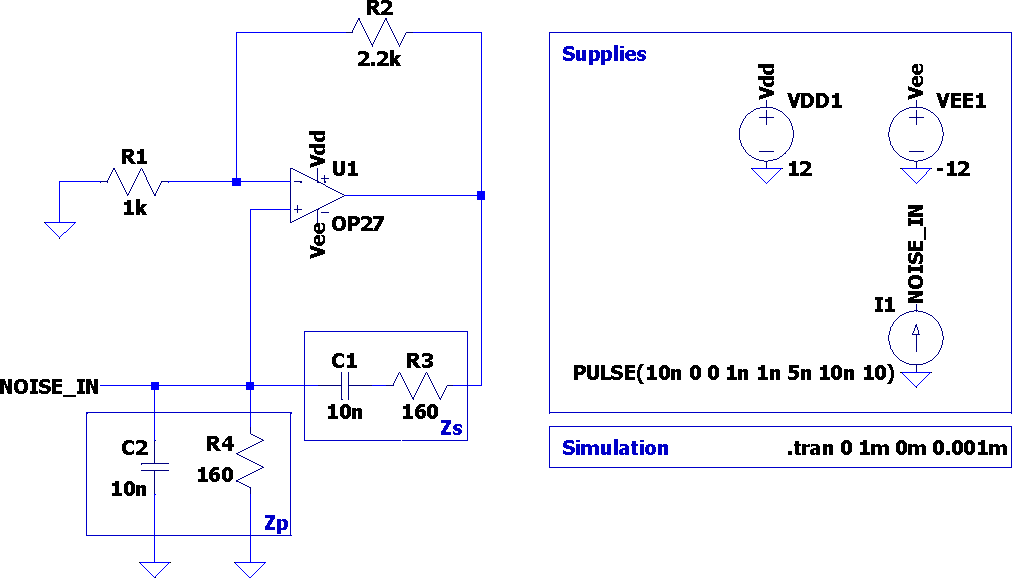
\includegraphics[width=0.7\linewidth]{wien/wien_ckt-crop}
		\caption{\textit{Left}: the Wien oscillator circuit. \textit{Right}: power supplies and SPICE directives used in the simulations.}
		\label{fig:wienckt}
	\end{figure}
	
	\noindent This oscillator is characterized by the transfer function \cite{sedra1998microelectronic}, \begin{align}
		L(s) & = \left(1 + \frac{R_2}{R_1}\right) \frac{Z_p}{Z_p + Z_s} \notag \\
			& = \frac{1 + R_2 / R_1}{3 + s RC + 1/sRC} \notag \\
		L(j\omega) & = \frac{1 + R_2 / R_1}{3 + j (\omega RC - 1 / \omega R C)} \label{eq:wientf}
	\end{align}
	From \eqref{eq:wientf}, the loop will create gain at a frequency $\omega_0$ with a unity gain $G$ as \begin{align*}
		\omega_0 & = 1 / RC \\
		G & = R_2 / R_1 = 2
	\end{align*}

	\subsubsection{Design}
	To follow the requirements, the Wien oscillator will be designed to generate the signal for the carrier frequency, between \SI{60}{\kHz} and \SI{80}{\kHz}, while allowing for the range of the input signal, which can reach \SI{4}{\kHz}. The Wien oscillator will be designed to output roughly \SI{70}{\kHz}. To accomplish this, it must be noted the relative ease of finding resistors of ranging values over the limited selection of capacitors. If a capacitance of \SI{10}{\nano\farad} is chosen, then from \eqref{eq:wientf}, the resistor in the feedback RC network must be roughly \SI{227}{\ohm}.
	
	For the feedback gain, given by $R_2/R_1$, a proportion of $2$ is required. For this, two common values were used, which would give an approximate gain of $2$: \begin{align*}
		R_1 & = \SI{1}{\kohm} \\
		R_2 & = \SI{2.2}{\kohm}
	\end{align*}
	After testing these values on-hardware, it was quickly realized that additional trimming of the resistor in the RC network. From testing, it was found that \SI{160}{\ohm} produced a oscillation at roughly \SI{72}{\kohm} with no load. With additional load, the frequency may drift up to \SI{74}{\kohm}, but that would be within the tolerances of the specifications.
		\vspace{-1em}
	\subsubsection{Simulation}
	% Transient/time oscillation
	% FFT
	Using LTspice, the circuit in Figure \ref{fig:wienckt} was simulated using a transient analysis to \SI{4}{\ms} in steps of \SI{0.1}{\us}. From the start, the simulation shows the gradual wind-up of the oscillator until it stabilizes after \SI{1}{\ms}, shown in Figure \ref{fig:wiensimt-crop}. After the oscillator stabilized, an FFT was generated showing a peak frequency of \SI{72}{\kHz} in Figure \ref{fig:wiensimfft-crop}.
		\vspace{-1em}
	\begin{figure}[h]
		\centering
		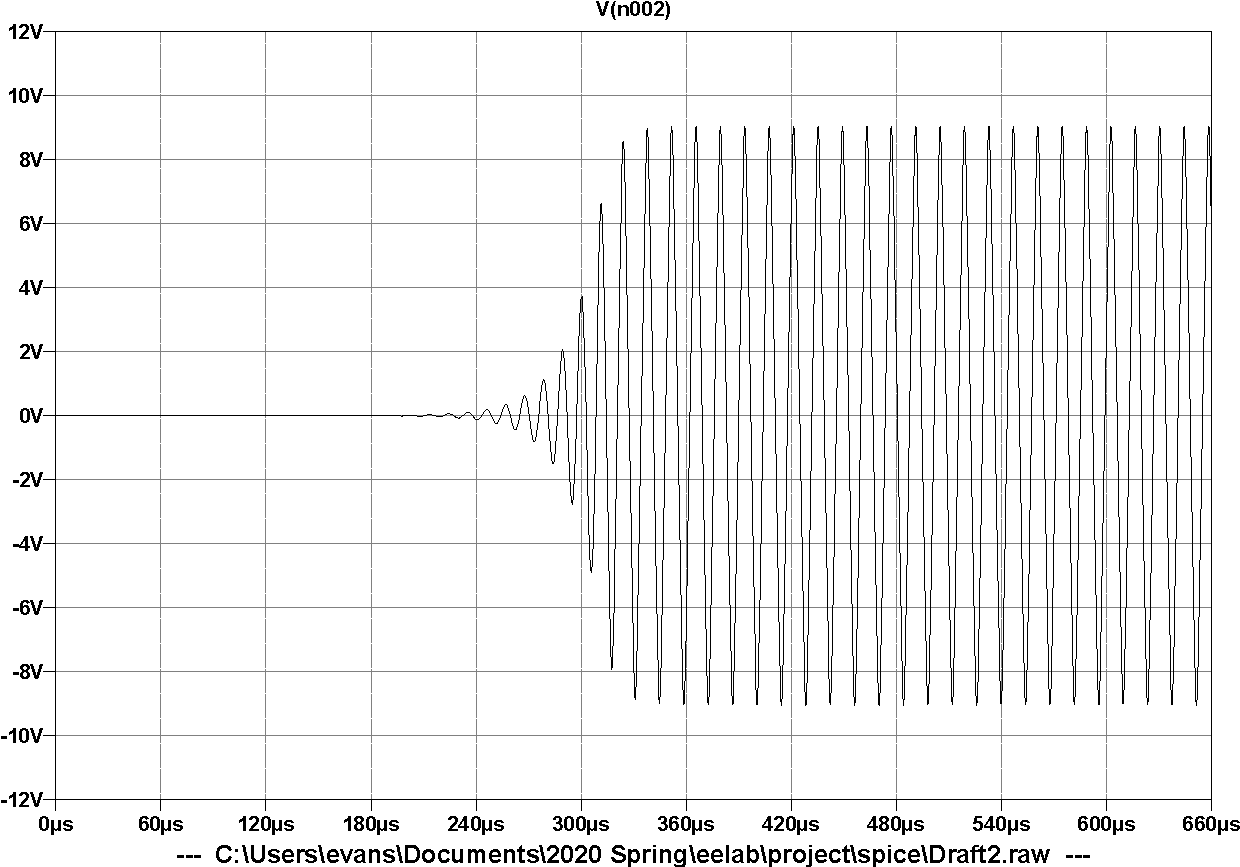
\includegraphics[width=0.6\linewidth,clip,trim=0 1.2em 0 0.9em]{wien/wien_simt-crop}
		\vspace{-0.5em}
		\caption{Transient simulation showing the start-up of the Wien oscillator.}
		\label{fig:wiensimt-crop}
	\end{figure}
	\vspace{-1.5em}
	\begin{figure}[h]
		\centering
		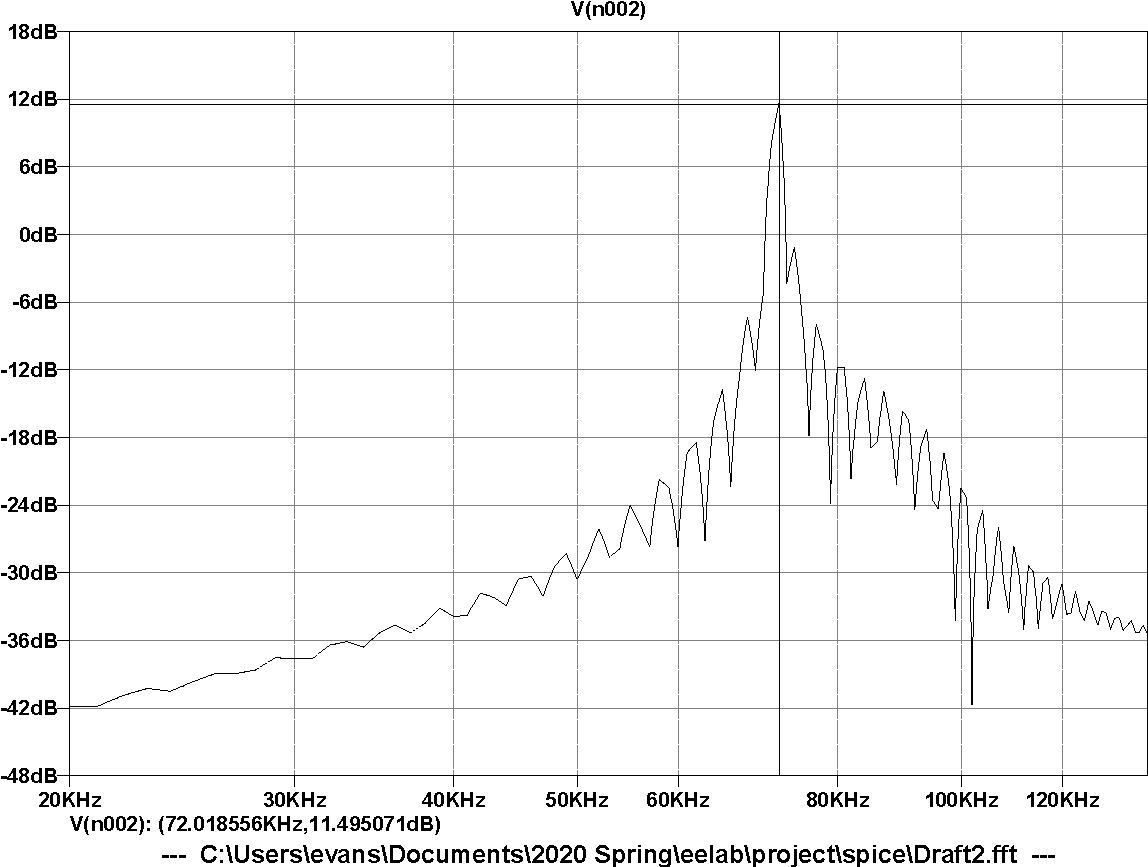
\includegraphics[width=0.6\linewidth,clip,trim=0 1.3em 0 0.9em]{wien/wien_simfft-crop}
		\vspace{-1em}
		\caption{An Fourier transform of the oscillator showing a peak frequency at roughly \SI{72}{\kHz}.}
		\label{fig:wiensimfft-crop}
	\end{figure}

	\clearpage %%%%%%%%%%%%%%%%%%%%%%%%%%%%%%%%%%%%%%%%%%%%%%%%%%%	
	\subsection{Switching Modulator}
	The switching modulator combines the carrier signal and the message signal. This is done simply through superposition of the two signals at the inverting terminal of the amplifier. Once the signals are added, the combined signal is amplified proportional to the input resistances of each signal. Lastly, a diode truncates the signal to the positive half.
	
	The circuit for the modulator is shown in Figure \ref{fig:modckt-crop} below, where the carrier signal is emulated using a sinusoidal input, \texttt{OSC\_IN}, and combined with the message signal, \texttt{LINE\_IN}. 
	% 109 673
	\begin{figure}[h]
		\centering
		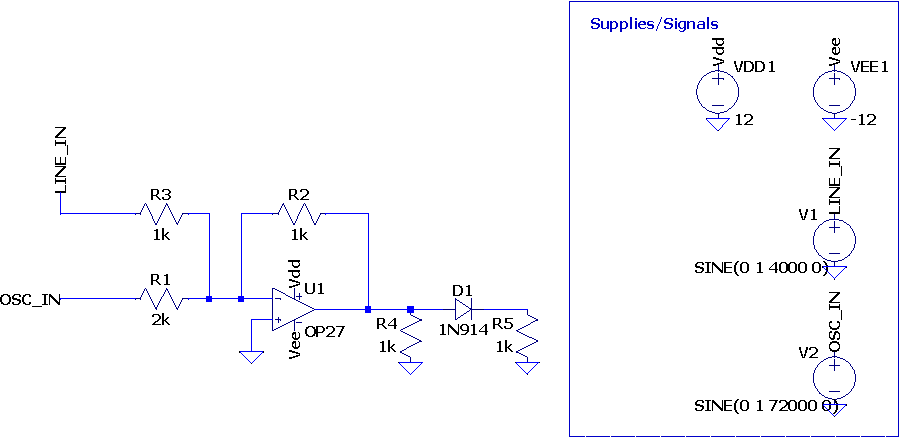
\includegraphics[width=0.7\linewidth]{modulator/modckt-crop}
		\caption{\textit{Left}: The circuit of the switching modulator. \textit{Right}: Power supplies and simulated signals.}
		\label{fig:modckt-crop}
	\end{figure}
	\subsubsection{Design}
	In the design shown in Figure \ref{fig:modckt-crop}, the carrier signal will have a half gain, given by the ratio of the resistors, $R_2 / R_1$. The message signal will have a unity gain, given by equal resistances of $R_2 / R_3$. These resistor ratios can be changed later on to adjust the modulation index of each input. In this design, the resistors can be chosen as \begin{align*}
		R_1 & = \SI{2}{\kohm} \\
		R_2 & = \SI{1}{\kohm} \\
		R_3 & = \SI{1}{\kohm}
	\end{align*}
	These resistors were chosen for the ease of finding \SI{1}{\kohm} resistors. Lastly, the signal will be clipped to the positive half using an 1N914 diode in a simple half-wave rectifier. 
	\subsubsection{Simulation}
	The modulator was simulated inline with the earlier \SI{72}{\kHz} Wien oscillator using an \SI{500}{\Hz} and \SI{4}{\kHz} message signal. The time-domain simulations for both message signals are shown in Figure \ref{fig:modouttime}. The Fourier transform of the output (pre-rectification) is shown in Figure \ref{fig:modfft}.
	
	\begin{figure}[h]
		\centering
		\begin{subfigure}{0.9\linewidth}
			\centering
			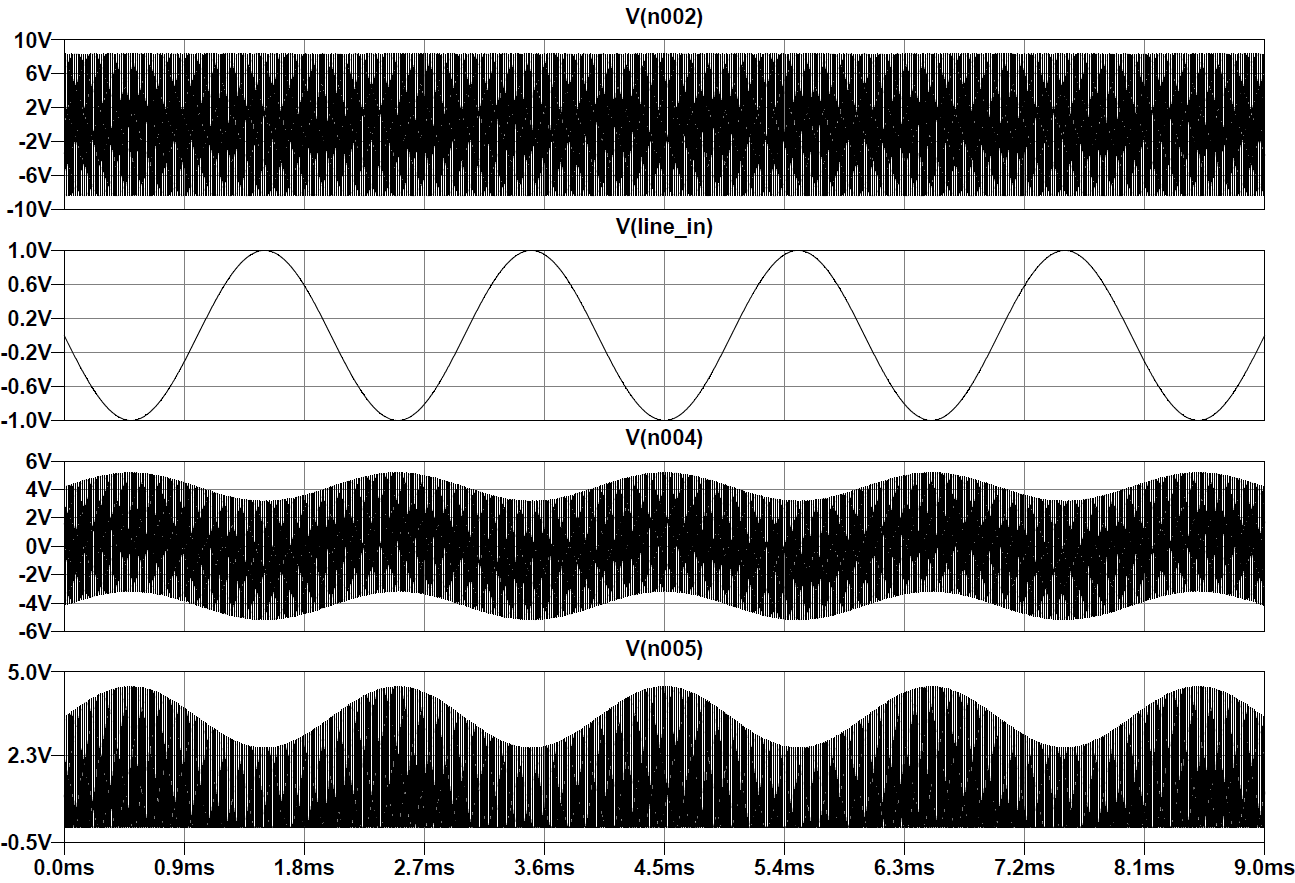
\includegraphics[width=\linewidth]{modulator/modout500img}
			\caption{Time simulation of modulator using the \SI{500}{\Hz} message signal.}
			\label{fig:modout500img}
		\end{subfigure}
				
		\begin{subfigure}{0.9\linewidth}
			\centering
			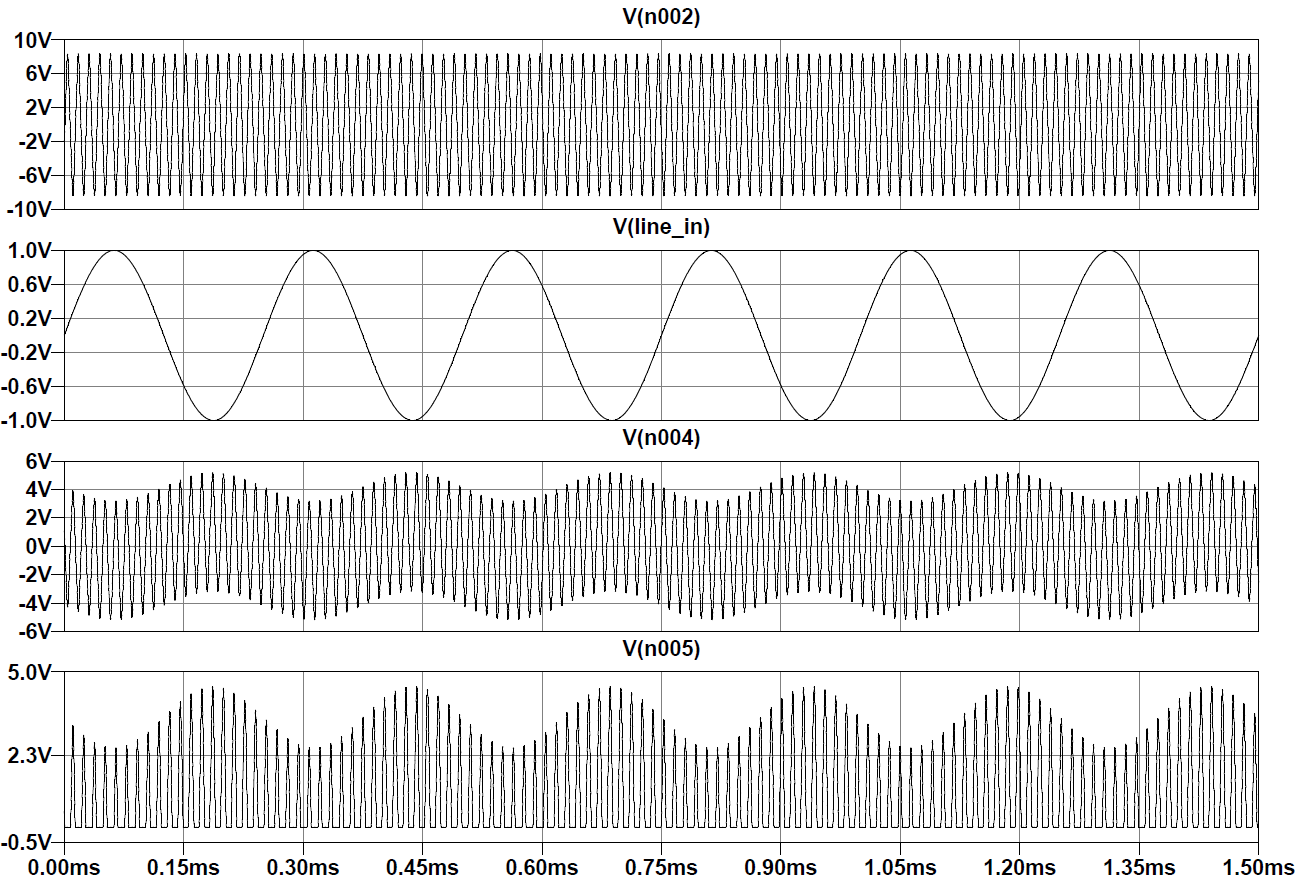
\includegraphics[width=\linewidth]{modulator/modout4kimg}
			\caption{Time simulation of modulator using the \SI{4}{\kHz} message signal.}
			\label{fig:modout4kimg}
		\end{subfigure}
		\caption{Time-domain simulation of the switching modulator using two message signals. Each figure contains: \textit{Topmost}: \SI{72}{\kHz} carrier signal input; \textit{Second}: Message signal input; \textit{Third}: Output of the summer; \textit{Last}: Output of the modulator after half-wave rectification.}
		\label{fig:modouttime}
	\end{figure}

	\begin{figure}[h]
		\centering
		\begin{subfigure}{0.9\linewidth}
			\centering
			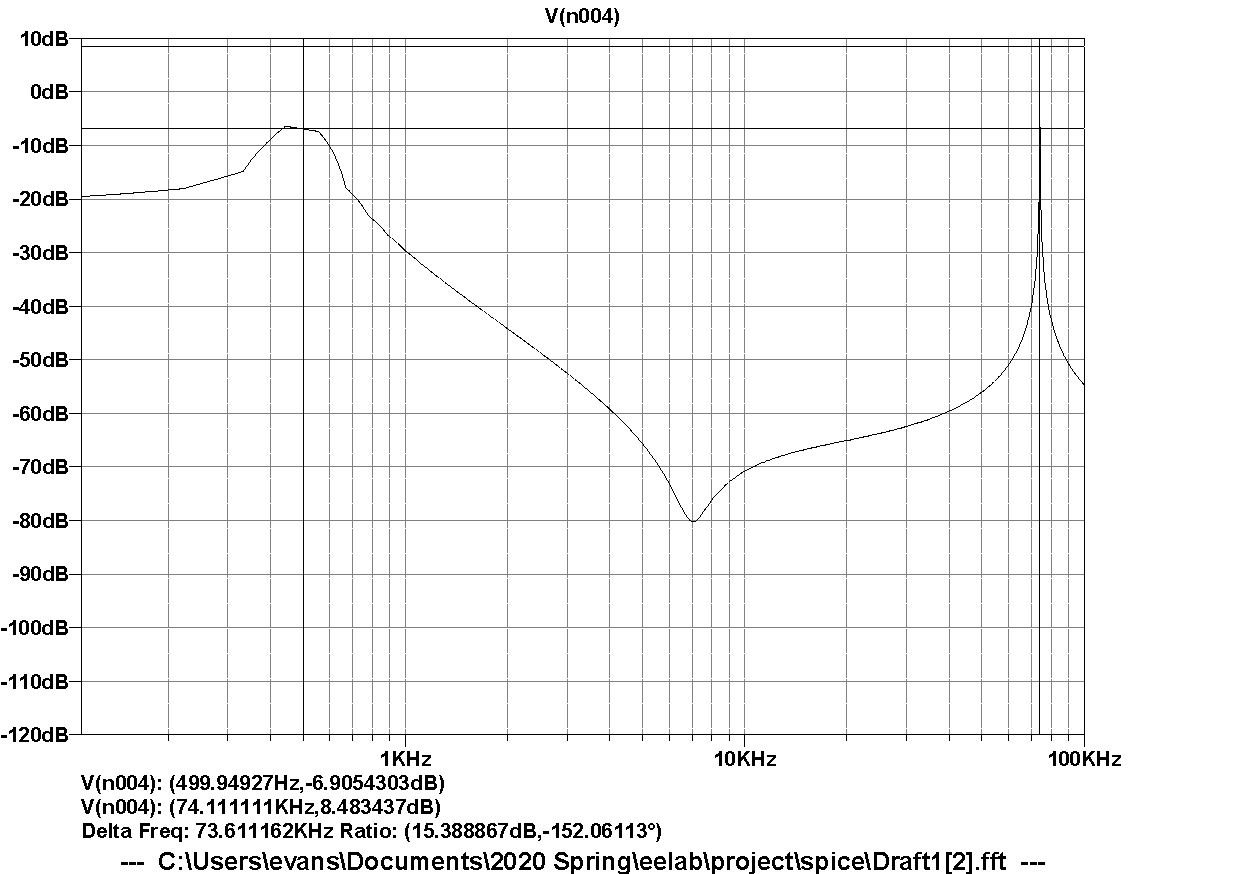
\includegraphics[width=\linewidth,clip,trim=0 1.2em 0 1.2em]{modulator/fft500}
			\caption{FFT of the output of the modulator with \SI{500}{\Hz} message signal.}
			\label{fig:fft500}
		\end{subfigure}
	
		\vspace{1em}
		
		\begin{subfigure}{0.9\linewidth}
			\centering
			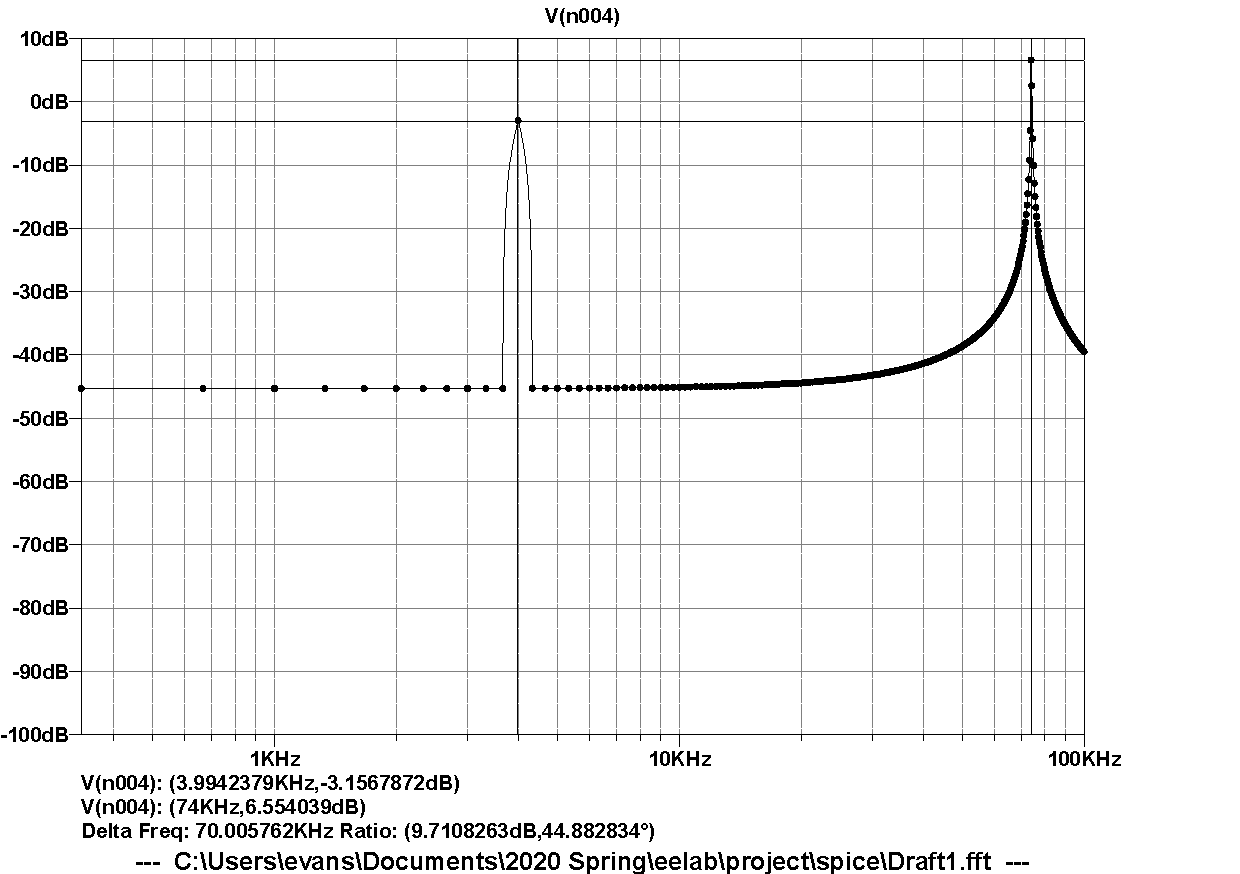
\includegraphics[width=\linewidth,clip,trim=0 1.2em 0 1.2em]{modulator/fft4k}
			\caption{FFT of the output of the modulator with \SI{4000}{\Hz} message signal.}
			\label{fig:fft4k}
		\end{subfigure}
	
		\caption{FFT of the output of the modulator for both message signal frequencies, showing peaks at the both the carrier signal and message signal frequencies.}
		\label{fig:modfft}
	\end{figure}

	\clearpage %%%%%%%%%%%%%%%%%%%%%%%%%%%%%%%%%%%%%%%%%%%%%%%%%%%		
	\subsection{High-Q Bandpass Filter}
	After modulation and half-wave rectification, the signal is passed to a high-Q bandpass filter to isolate the range of the combined carrier and message signal. Effectively, the output signal now becomes an amplitude modulated wave with an envelope vertically symmetric. The circuit of the filter used in this project is shown in Figure \ref{fig:highqbpfckt-crop} below.
		% nilssonriedel
	\begin{figure}[h]
		\centering
		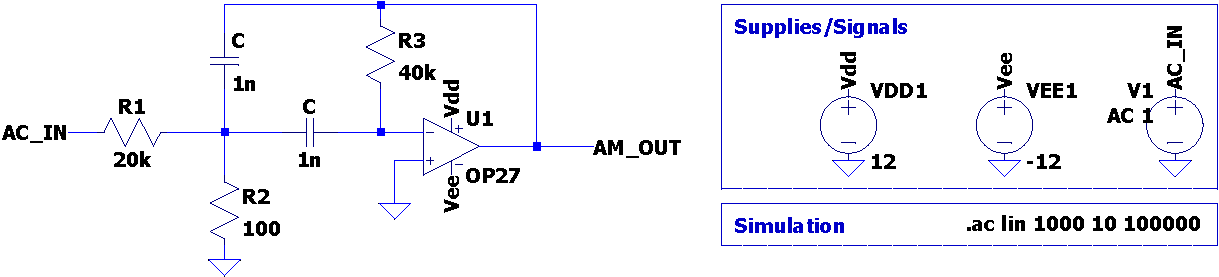
\includegraphics[width=0.9\linewidth]{highqbpf/highqbpfckt-crop}
		\caption{\textit{Left}: The high quality bandpass filter used in the radio project. \textit{Right}: The voltage sources and simulation SPICE directive.}
		\label{fig:highqbpfckt-crop}
	\end{figure}
	
	For this filter, its transfer function can be determined by finding the impedances throughout this non-inverting op-amp configuration. It can be shown\cite{nilssonriedel} that the transfer function is \begin{align*}
		H(s) & = \frac{-K\beta}{s^2 + \beta s + \omega_0^2}
		\intertext{Where the center frequency $\omega_0$ and bandwidth $\beta$ is given as}
		\omega_0 & = \frac{1}{\left(R_1 \parallel R_2\right) R_3 C^2} \\
		\beta & = 2 \pi \left(2 \times 4000\right) \\
			& = \frac{2}{R_3 C} = \frac{1}{K R_1 C}
	\end{align*}
	
	\subsubsection{Design}
	For this, a MATLAB script was used to iteratively find potential combinations of component values and is included in Snippet \ref{lst:highqbpf} (Appendix A). The capacitances were fixed to \SI{1}{\nano\farad} as there are many ceramic capacitors of this value available. Initially, $R_1$ and $R_3$ were calculated to an exact value of \SI{19.894}{\kohm} and \SI{39.789}{\kohm} respectively. As there are an abundance of \SI{10}{\kohm} resistors and multiples, these resistances were rounded to \SI{20}{\kohm} and \SI{40}{\kohm}. 

	After fixing these component values, $R_2$ was iteratively determined as \SI{119}{\ohm} by testing different $R_2$ values and calculating the center frequency. After simulating these values, it was realized that $R_2$ must be trimmed to \SI{100}{\ohm}, likely due to internal capacitance of the op-amp affecting the center frequency.
	
	\subsubsection{Simulation}
	The filter was initially simulated using a linear AC sweep. The frequency response is shown in Figure \ref{fig:highqbpfsweep}. Next, the filter was placed at the output of the switching modulator and the two message frequencies were tested. The time-domain simulation is shown in Figure \ref{fig:highqt}. For the time-domain responses, the FFT showing the two peaks at $f_c \pm f_m$ is shown in Figure \ref{fig:highqfft}.

	\begin{figure}[h]
		\centering
		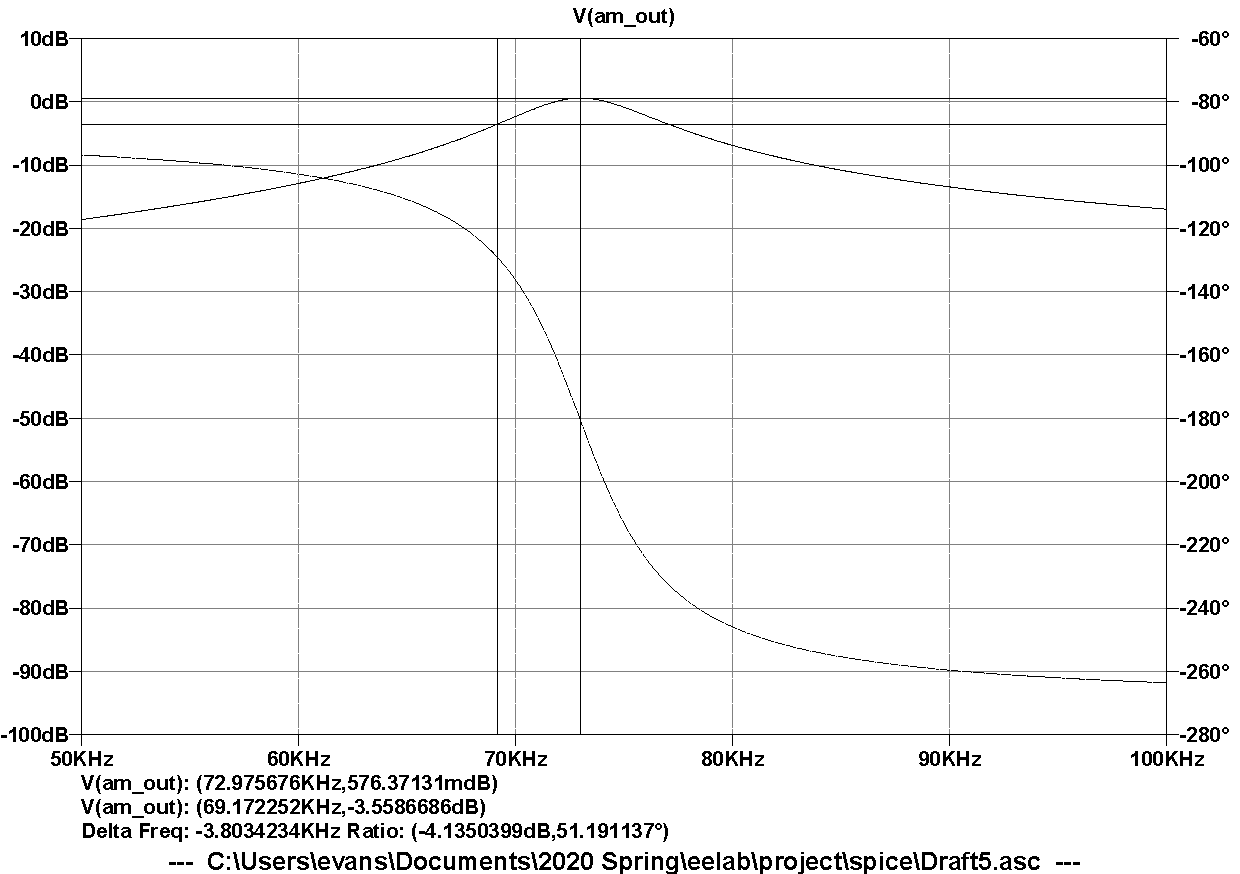
\includegraphics[width=\linewidth,clip,trim=0 1.1em 0 1.2em]{highqbpf/highqbpfsweep}
		\caption{Simulated bode plot of the frequency response of the high Q bandpass filter.}
		\label{fig:highqbpfsweep}
	\end{figure}

	\clearpage
	\begin{figure}[h]	
		\centering
		\begin{subfigure}{\linewidth}
			\centering
			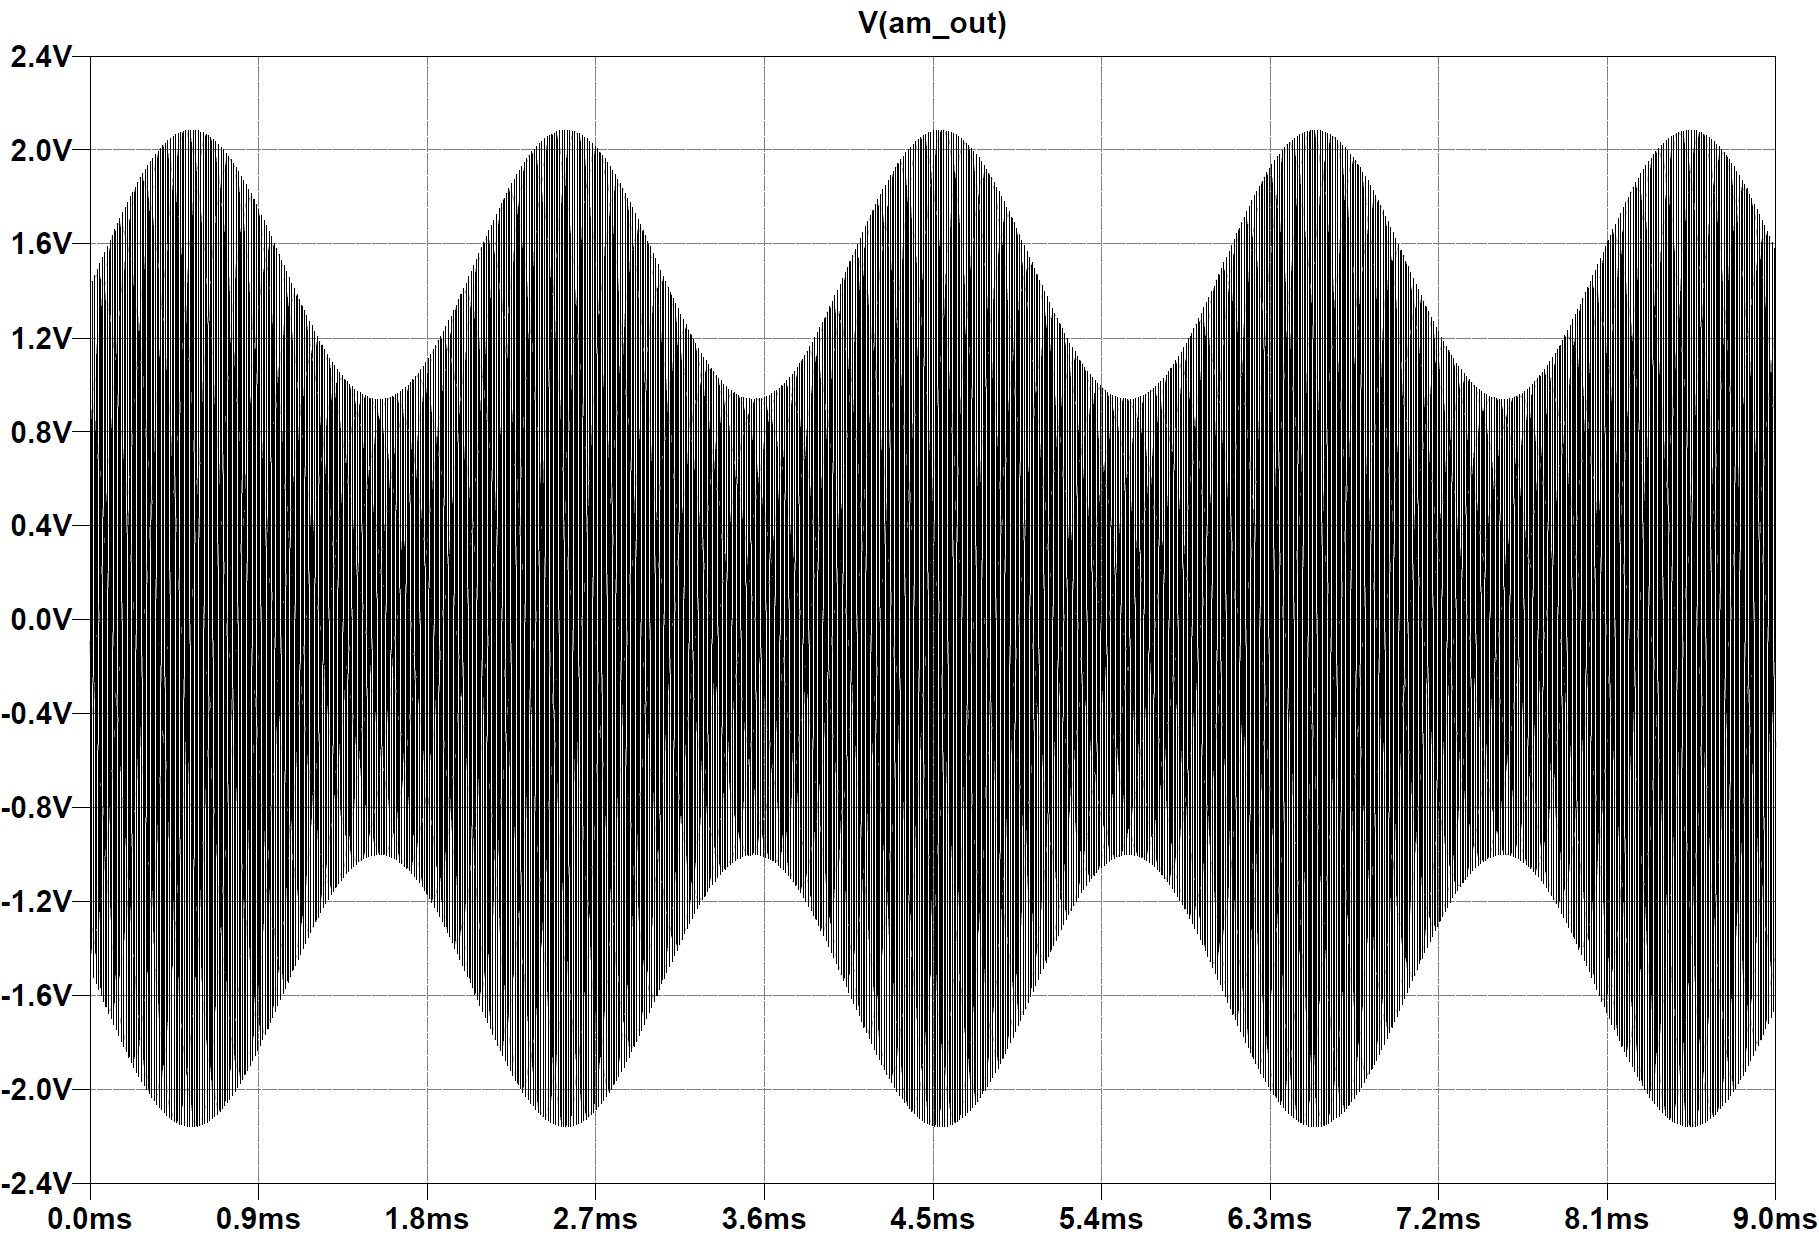
\includegraphics[width=0.9\linewidth]{highqbpf/highqt500img}
			\caption{}
			\label{fig:highqt500img}
		\end{subfigure}
		\vspace{1em}
			
		\begin{subfigure}{\linewidth}
			\centering
			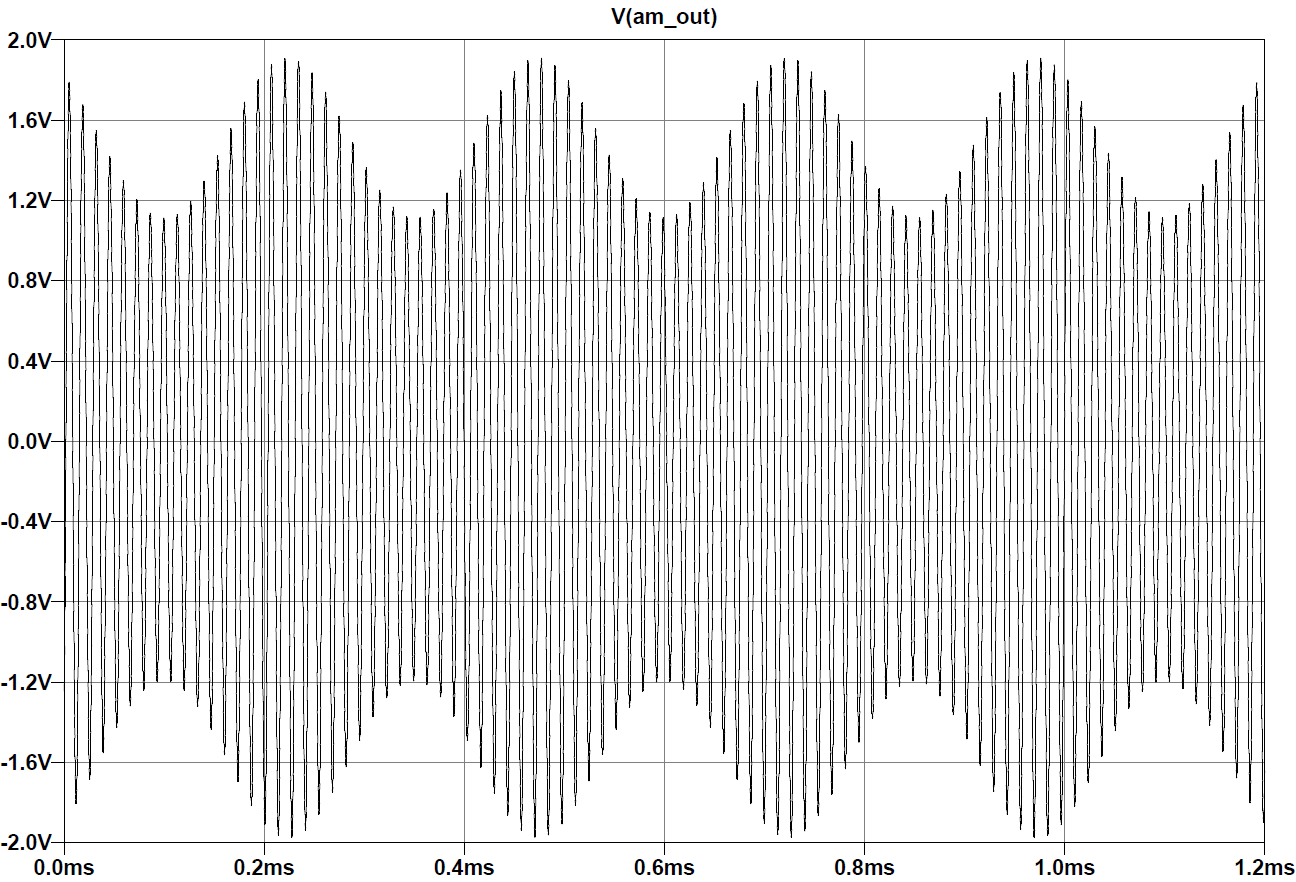
\includegraphics[width=0.9\linewidth]{highqbpf/highqt4kimg}
			\caption{}
			\label{fig:highqt4kimg}
		\end{subfigure}

		\caption{Time-domain responses of the high-Q bandpass filter for message signals of (a) \SI{500}{\Hz}, (b) \SI{4}{\kHz}.}
		\label{fig:highqt}
	\end{figure}


	\begin{figure}[h]
		\centering
		\begin{subfigure}{\linewidth}
			\centering
			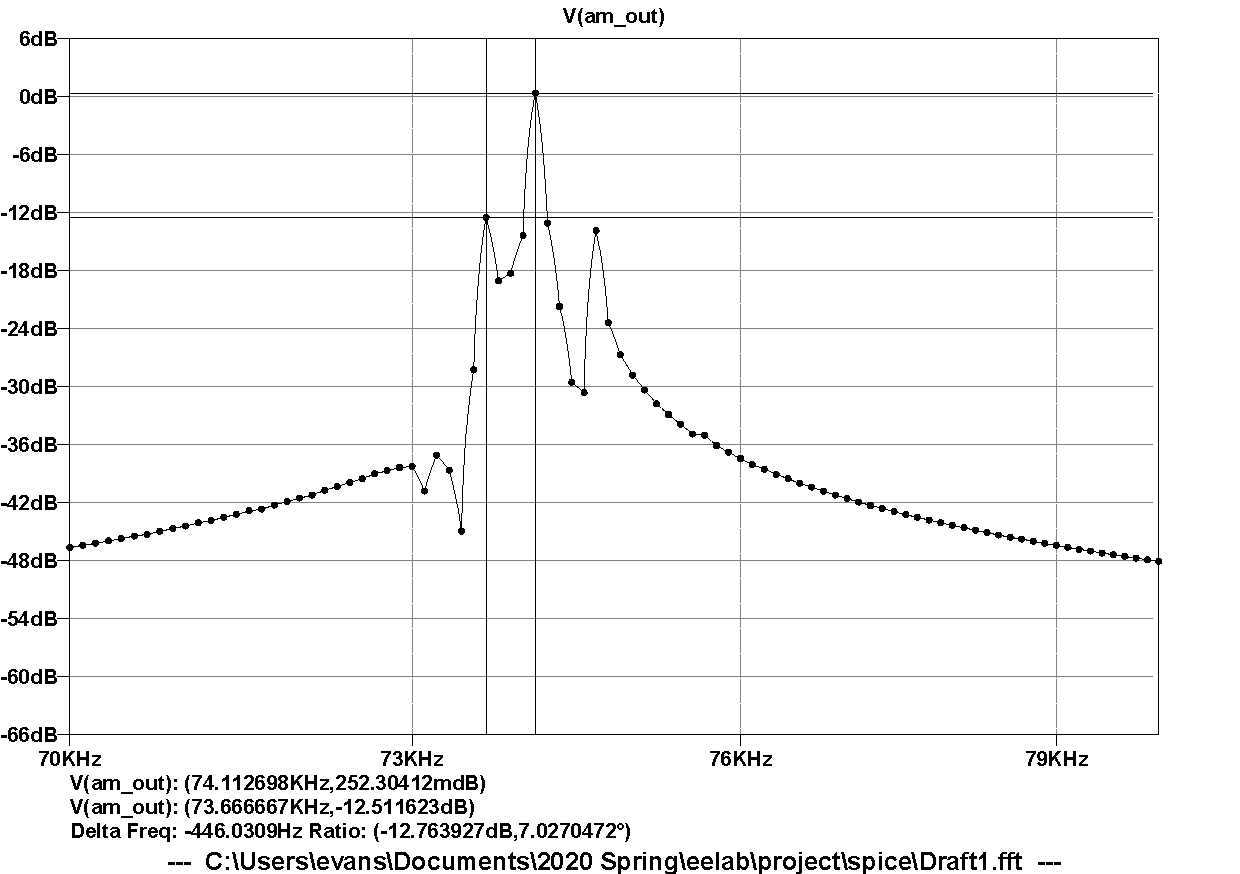
\includegraphics[width=0.9\linewidth,clip,trim=0 1.1em 0 1.2em]{highqbpf/highqfft500}
			\caption{}
			\label{fig:highqfft500}
		\end{subfigure}
		
		\begin{subfigure}{\linewidth}
			\centering
			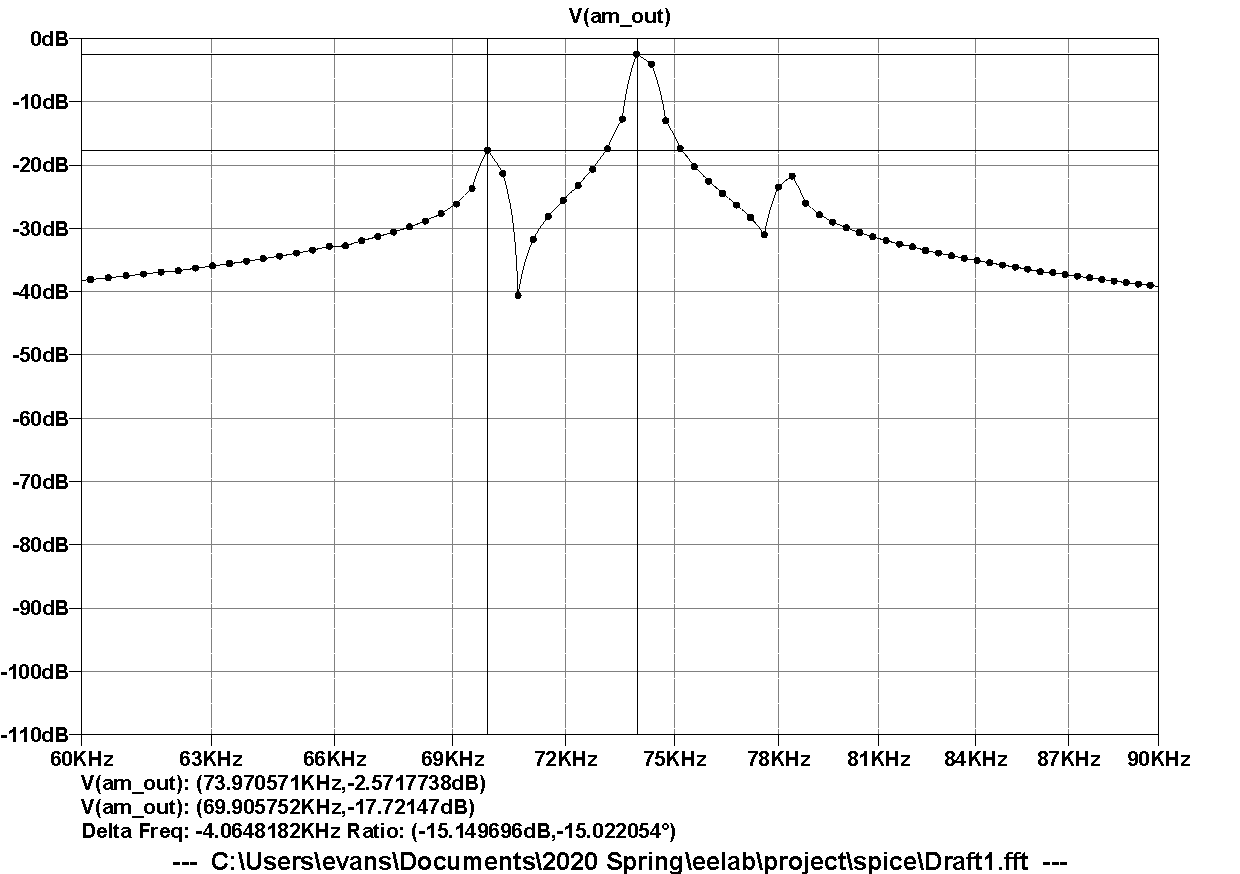
\includegraphics[width=0.9\linewidth,clip,trim=0 1.1em 0 1.2em]{highqbpf/highqfft4k}
			\caption{}
			\label{fig:highqfft4k}
		\end{subfigure}
		
		\caption{Frequency-domain responses of the high-Q bandpass filter for message signals of (a) \SI{500}{\Hz}, (b) \SI{4}{\kHz}.}
		\label{fig:highqfft}
	\end{figure}

	\clearpage %%%%%%%%%%%%%%%%%%%%%%%%%%%%%%%%%%%%%%%%%%%%%%%%%%%	
	\subsection{Power Amplifier}
	The power amplifier in this project amplifies the AM signal and provides a way to drive a high-power output, such a low-impedance BNC cable and receiver. In this design, an op-amp is used to drive the complementary BJTs with the output providing negative feedback into the op-amp. The circuit is shown below in Figure \ref{fig:powerampckt-crop}, with the amplification provided by the usual inverting op-amp gain, $-R_2 / R_1$.
	
	\begin{figure}[h]
		\centering
		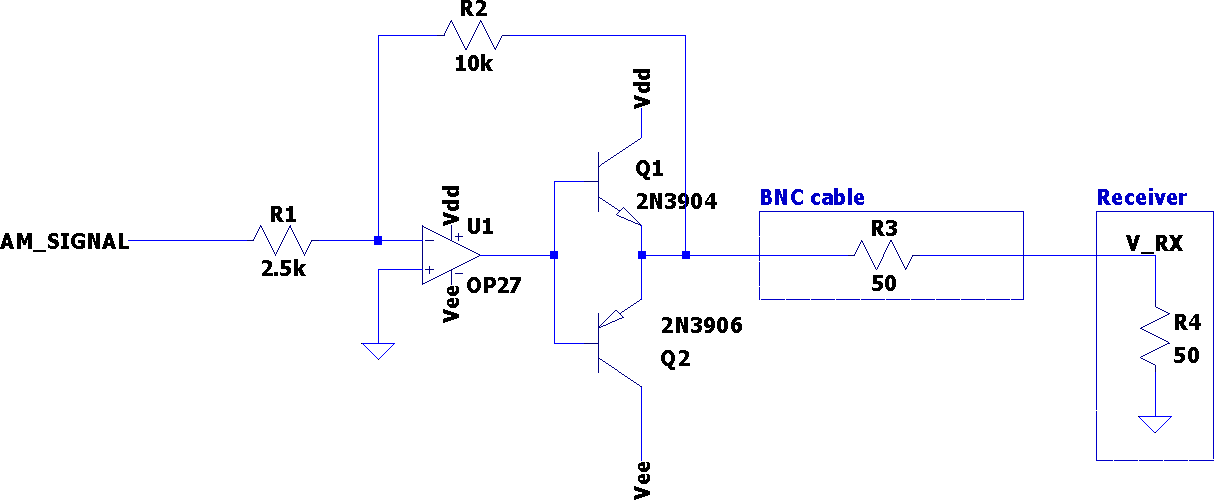
\includegraphics[width=0.7\linewidth]{poweramp/powerampckt-crop}
		\caption{Circuit of the power amplifier used in the AM radio.}
		\label{fig:powerampckt-crop}
	\end{figure}
	
	\subsubsection{Design}
	Given the limits of the power supply and the maximum swings of the input signals, a message voltage peak-to-peak \SI{1.5}{\V} will be aimed for. Through several iterations in LTspice, the resistors were chosen as \begin{align*}
		R_1 & = \SI{2.5}{\kohm} \\
		R_2 & = \SI{10}{\kohm}
	\end{align*}
	
	\subsubsection{Simulation}
	Simulating this in the time-domain, Figure \ref{fig:poweramp}, shows a peak output of roughly \SI{8}{\V} prior to the BNC cable impedance. As the voltage divider of the BNC cable and receiver halves the voltage, the magnitude at the receiver is \SI{4}{\V}. The envelope message signal is then approximately \SI{1.5}{\V} to \SI{2.5}{\V} in magnitude.
	
	\begin{figure}[h]	
		\centering
		\begin{subfigure}{\linewidth}
			\centering
			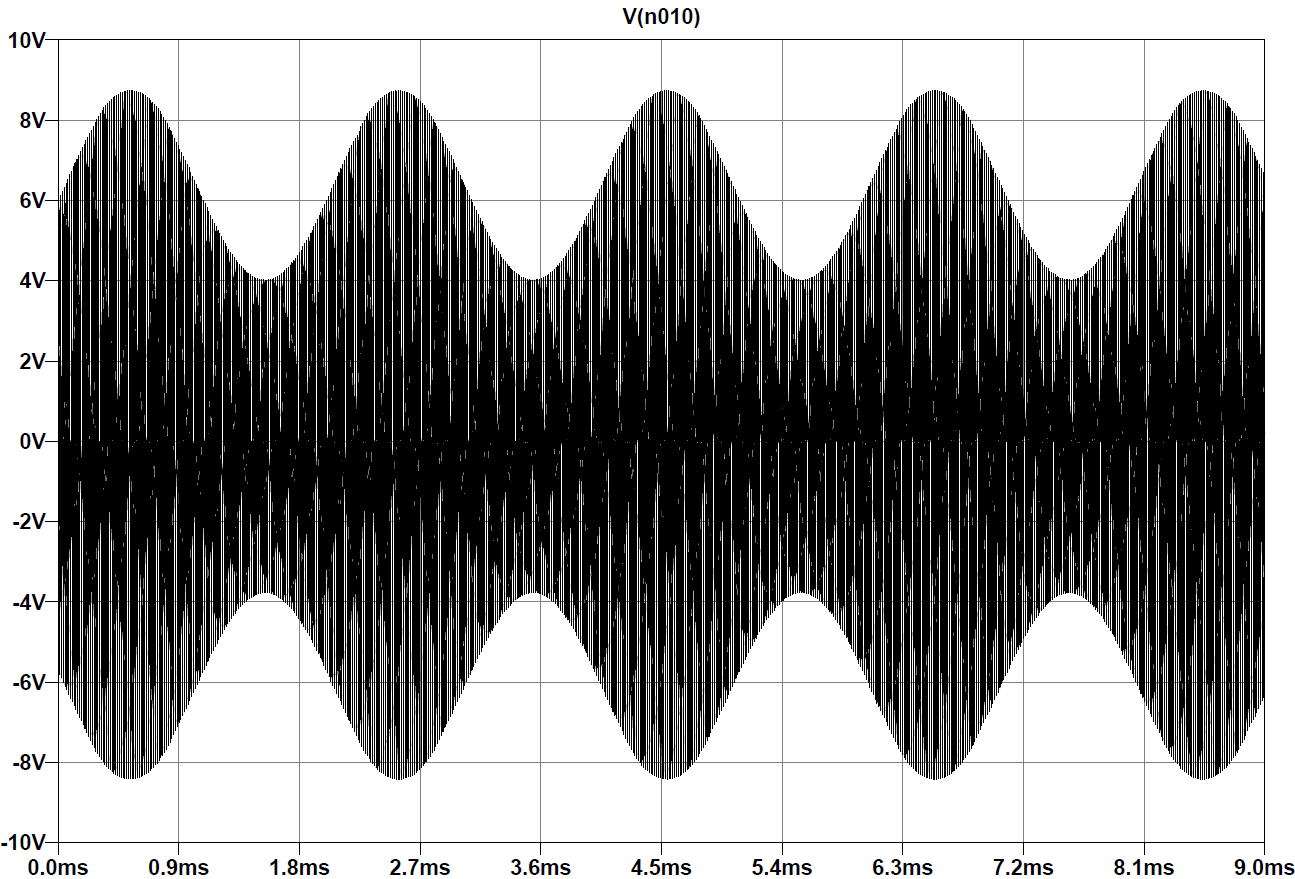
\includegraphics[width=0.9\linewidth]{poweramp/poweramp500img}
			\caption{}
			\label{fig:poweramp500img}
		\end{subfigure}
		
		\begin{subfigure}{0.9\linewidth}
			\centering
			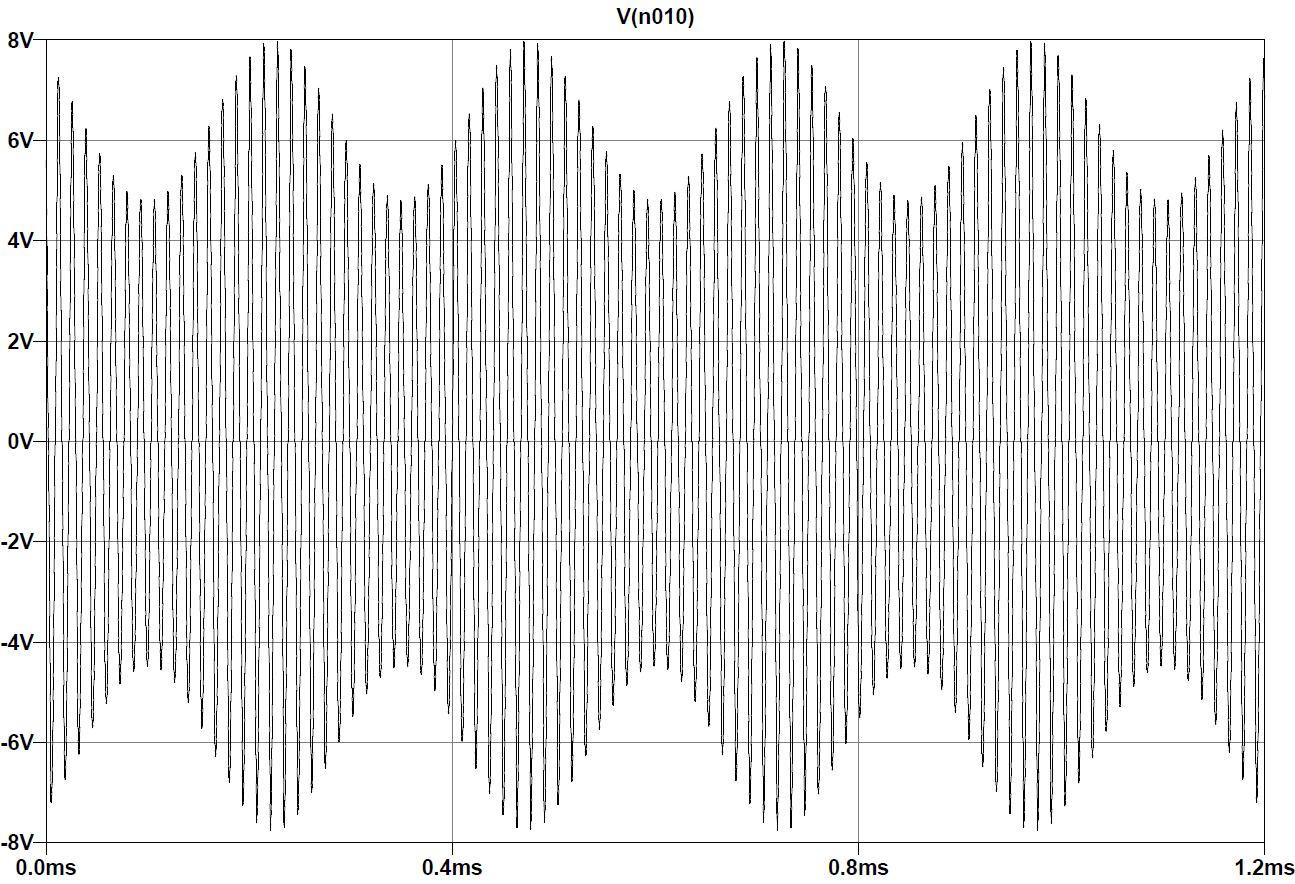
\includegraphics[width=\linewidth]{poweramp/poweramp4kimg}
			\caption{}
			\label{fig:poweramp4kimg}
		\end{subfigure}
		
		\caption{Output of the power amplifier for message signals of (a) \SI{500}{\Hz}, (b) \SI{4}{\kHz}.}
		\label{fig:poweramp}
	\end{figure}

	\clearpage %%%%%%%%%%%%%%%%%%%%%%%%%%%%%%%%%%%%%%%%%%%%%%%%%%%	
	\subsection{Peak Detector}
	After the receiver, the message signal must be separated from the carrier wave. To accomplish this, a peak detector will be used, which will find peaks within the carrier signal, in turn giving a rough outline of the message signal.
	
	A simple peak detector circuit will use a diode and an RC network on the cathode-side. When the input voltage swings upward, current will pass through the diode and will charge the capacitor at an equal voltage. On the negative swings, the voltage is retained by the capacitor and the diode will be reverse biased, and no current will pass through initially. While in reverse bias, the resistor will begin to drain the capacitor until the next peak detection.
	
	The circuit used is shown in Figure \ref{fig:peakckt} with a buffer on its output. Since the time constant of an RC network is given as \begin{align}
		\tau & = RC \label{eq:taurc}
		\intertext{We can determine an ideal $R$ and $C$ values based on the rise and fall time of the signal peaks. At a maximum potential difference between two peaks, an ideal time constant value can be determined as}
		V_1 & = V_0 \; e^{-\Delta T / \tau} \notag \\
		\tau & = -\Delta T / \ln(V_1 / V_0) \notag \\
			& = - 1 / \left[f_c \ln(V_1 / V_0) \right] \label{eq:peakdetect}
	\end{align}
	
	\begin{figure}[h]
		\centering
		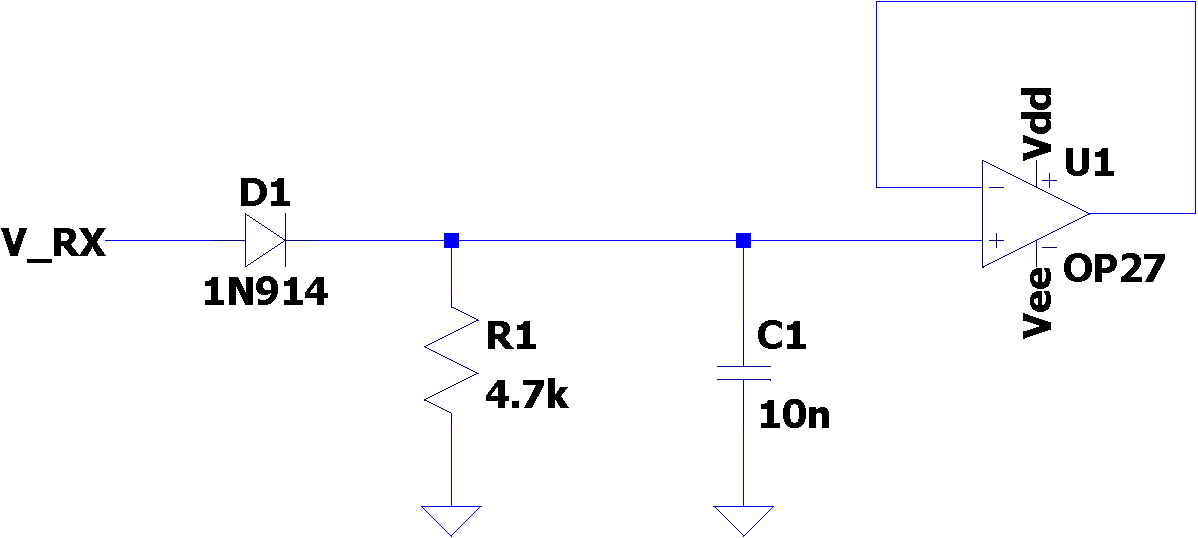
\includegraphics[width=0.6\linewidth]{peak/peakckt-crop}
		\caption{A peak detector circuit and output buffer.}
		\label{fig:peakckt}
	\end{figure}
	
	\subsubsection{Design}
	From simulating the power amplifier, the output has the highest difference in peak values of \SI{2.95}{\V} and \SI{2.71}{\V}. If a capacitor value of \SI{10}{\nano\farad} is used, then an ideal resistor value can be found using \eqref{eq:taurc} and \eqref{eq:peakdetect}, \begin{align*}
		\tau & = \SI{159.3}{\us} = RC \\
		R_\mathrm{max} & = \frac{\num{159.3e-6}}{\num{10e-9}} \approx \SI{16}{\kohm}
	\end{align*}
	This resistance value gives an estimate of the maximum resistance needed. Any higher will prevent additional peaks from being detected, and lower resistance values will create additional noise to later filter. Here, it is best to err on the side of caution and choose a much lower resistance of \SI{4.7}{\kohm}. Although doing so will create noise, it can easily be filtered out using a low-pass filter, allowing only the low-frequency message signal through.
	
	\subsubsection{Simulation}
	The peak detector was simulated on the full project circuit with both the \SI{500}{\Hz} and \SI{4}{\kHz} signal in the time domain, shown in Figure \ref{fig:peaks}. For both message frequencies, there is a minimum of \SI{180}{\mV} of allowance as the voltage falls between peaks.
	
	\vfil
	
	\begin{figure}[h]	
		\begin{subfigure}{\linewidth}
			\centering
			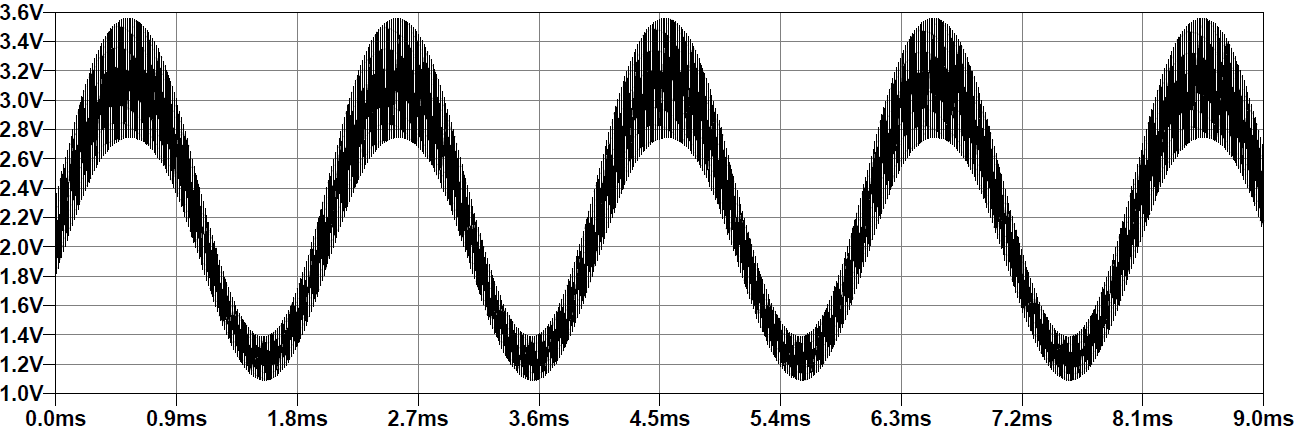
\includegraphics[width=\linewidth]{peak/peak500img}
			\caption{}
			\label{fig:peak500img}
		\end{subfigure}
		
		\vspace{2em}
		
		\begin{subfigure}{\linewidth}
			\centering
			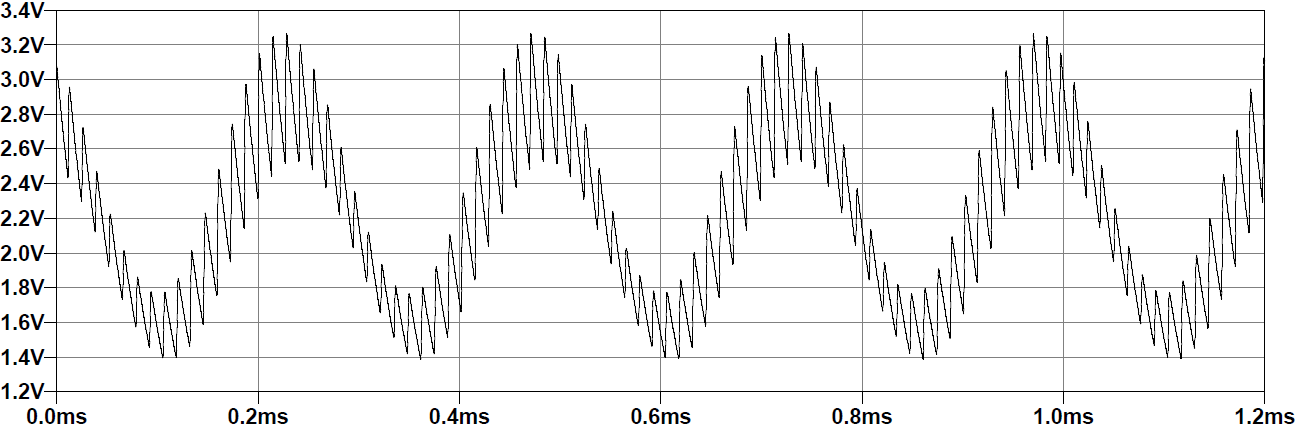
\includegraphics[width=\linewidth]{peak/peak4kimg}
			\caption{}
			\label{fig:peak4kimg}
		\end{subfigure}
		
		\caption{Output of the peak detector for message signals of (a) \SI{500}{\Hz}, (b) \SI{4}{\kHz}.}
		\label{fig:peaks}
	\end{figure}

	\clearpage %%%%%%%%%%%%%%%%%%%%%%%%%%%%%%%%%%%%%%%%%%%%%%%%%%%	
	\subsection{Bandpass Filter}
	The peak detector outputs significant noise must be filtered out. A second-order Butterworth low- and high-pass filter will be used to remove noise generated by the peak detector, as well as any other noise on the signal. It can be shown\cite{nilssonriedel} that the transfer function of a Butterworth low- and high-pass filters shown in Figure \ref{fig:bpfckt-crop} are given as \begin{align}
		H_\mathrm{LP}(s) & = \frac{\omega_{c1} ^2}{s^2 + 2 \zeta \omega_{c1} s + \omega_{c1}^2} = \frac{ 1 / C_1 C_2 R^2 }{s^2 + \frac{2}{R C_1}s + \frac{1}{C_1 C_2 R^2}} \label{eq:hlp} \\
		H_\mathrm{HP}(s) & = \frac{s^2}{s^2 + 2 \zeta \omega_{c2} s + \omega_{c2}^2} = \frac{s^2}{s^2 + \frac{2}{R_2 C} s + \frac{1}{R_1 R_2 C^2}} \label{eq:hhp}
	\end{align}
	
	\begin{figure}[h]
		\centering
		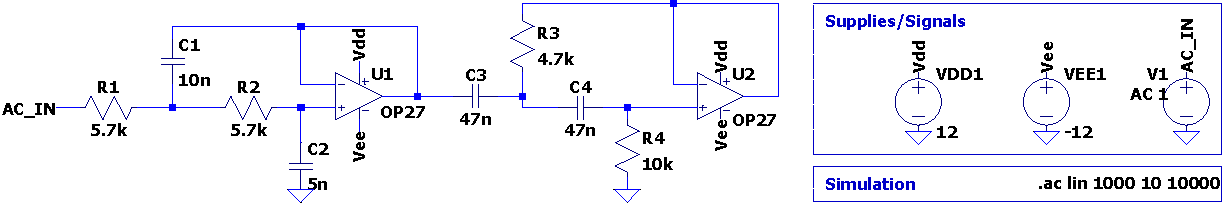
\includegraphics[width=1\linewidth]{bpf/bpfckt-crop}
		\caption{The two Butterworth filters used to filter the output of the peak detector.}
		\label{fig:bpfckt-crop}
	\end{figure}

	\subsubsection{Design}
	As the message signal is limited to \SI{500}{\Hz} to \SI{4}{\kHz}, the capacitor values can be chosen arbitrarily and used to calculate the resistances for those cutoff frequencies using \eqref{eq:hlp} and \eqref{eq:hhp}. For the low-pass filter, the cutoff frequency is \SI{4}{\kHz}. Then, choosing \SI{10}{\nano\farad} as first capacitor value, then \begin{align*}
		2 \zeta \omega_{c1} & = 2 \times 0.707 \times 2 \pi 4000 \\
			& = \frac{2}{R C_1} = \frac{2}{R \times \num{10e-9}} \\
		R & \approx \SI{5.7}{\kohm} \\
		\omega_{c1}^2 & = \frac{1}{C_1 C_2 R^2} = \frac{1}{\num{10e-9} \times C_2 \times \left(\num{5.7e3}\right)^2} \\
		C_2 & \approx \SI{5}{\nano\farad}
	\end{align*}
	Taking a similar approach for the high-pass filter and the low-frequency cutoff of \SI{500}{\Hz}, \begin{align*}
		2 \zeta \omega_{c2} & = 2 \times 0.707 \times 2 \pi 500 \\
			& = \frac{2}{R_2 C} = \frac{2}{\num{47e-9} \times R_2} \\
		R_2 & = \SI{9.58}{\kohm} \approx \SI{10}{\kohm} \\
		R_1 & \approx \SI{4.7}{\kohm}
	\end{align*}
	
	\clearpage
	\subsubsection{Simulation}
	In this simulation, an AC sweep was used to determine how effective the filter was at removing frequencies outside of the expected bandwidth. The bode plot is shown below in Figure \ref{fig:bpfresp}. After attaching the filter to the AM radio circuit, a time-domain simulation was done for both message frequencies. These are shown in Figure \ref{fig:bpfout}, displaying a sine wave with little distortion near the proper frequencies.
	
	\vfil 
	
	\begin{figure}[h]
		\centering
		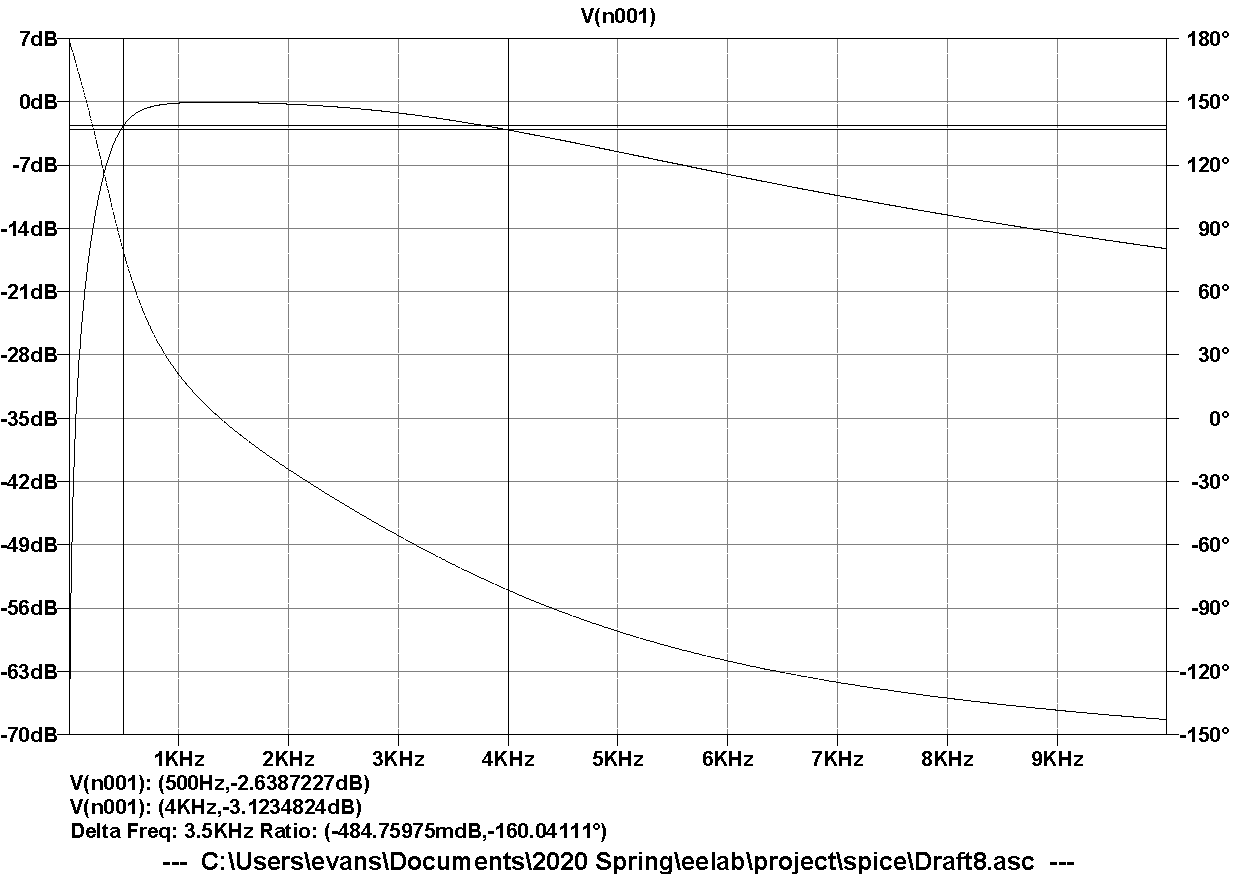
\includegraphics[width=\linewidth,clip,trim=0 1.1em 0 1.2em]{bpf/bpfresp}
		\caption{Simulated bode plot of the frequency response of the high Q bandpass filter.}
		\label{fig:bpfresp}
	\end{figure}

	\begin{figure}[h]
		\centering
		\begin{subfigure}{0.9\linewidth}
			\centering
			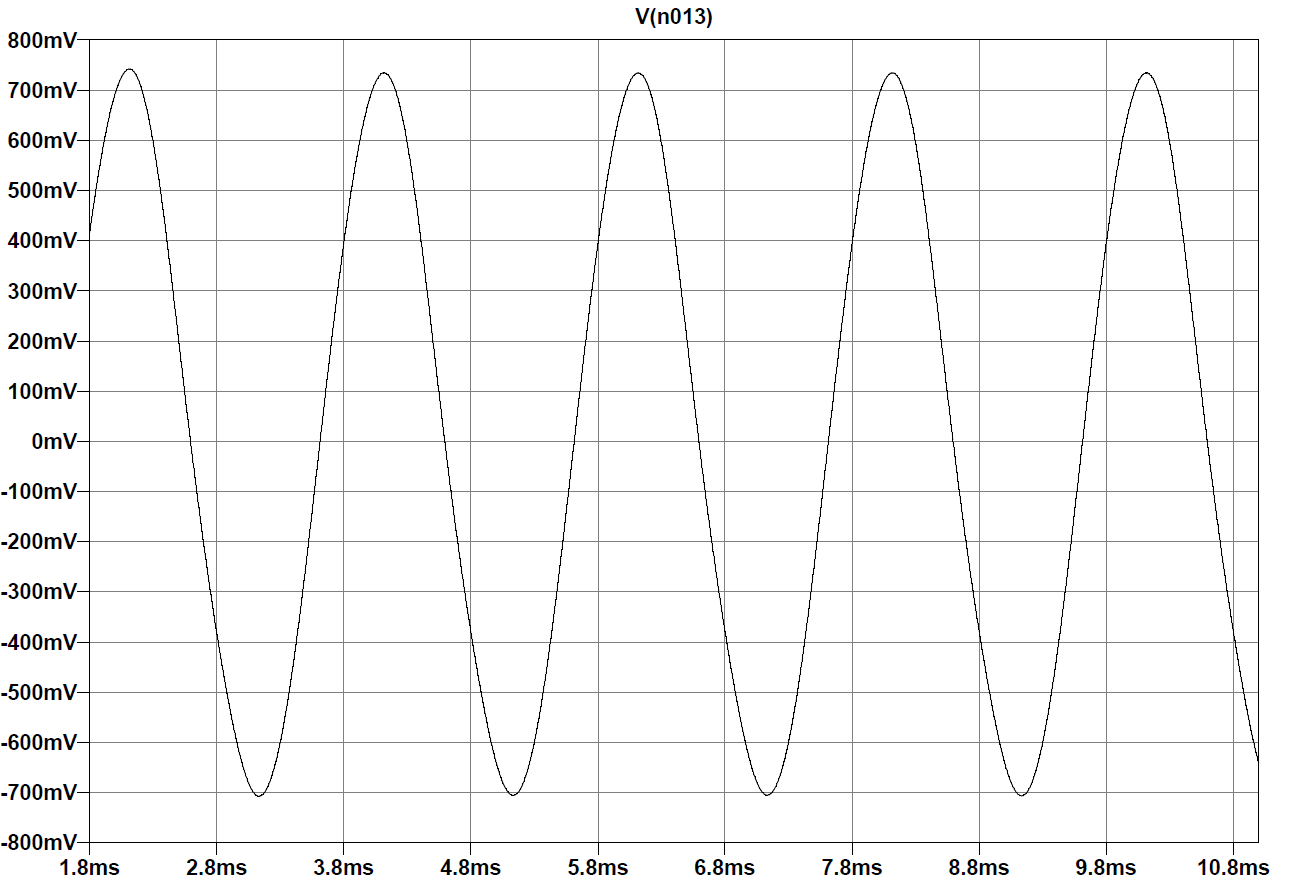
\includegraphics[width=\linewidth]{bpf/bpf500hz}
			\caption{}
			\label{fig:bpf500hz}
		\end{subfigure}
		
		\begin{subfigure}{0.9\linewidth}
			\centering
			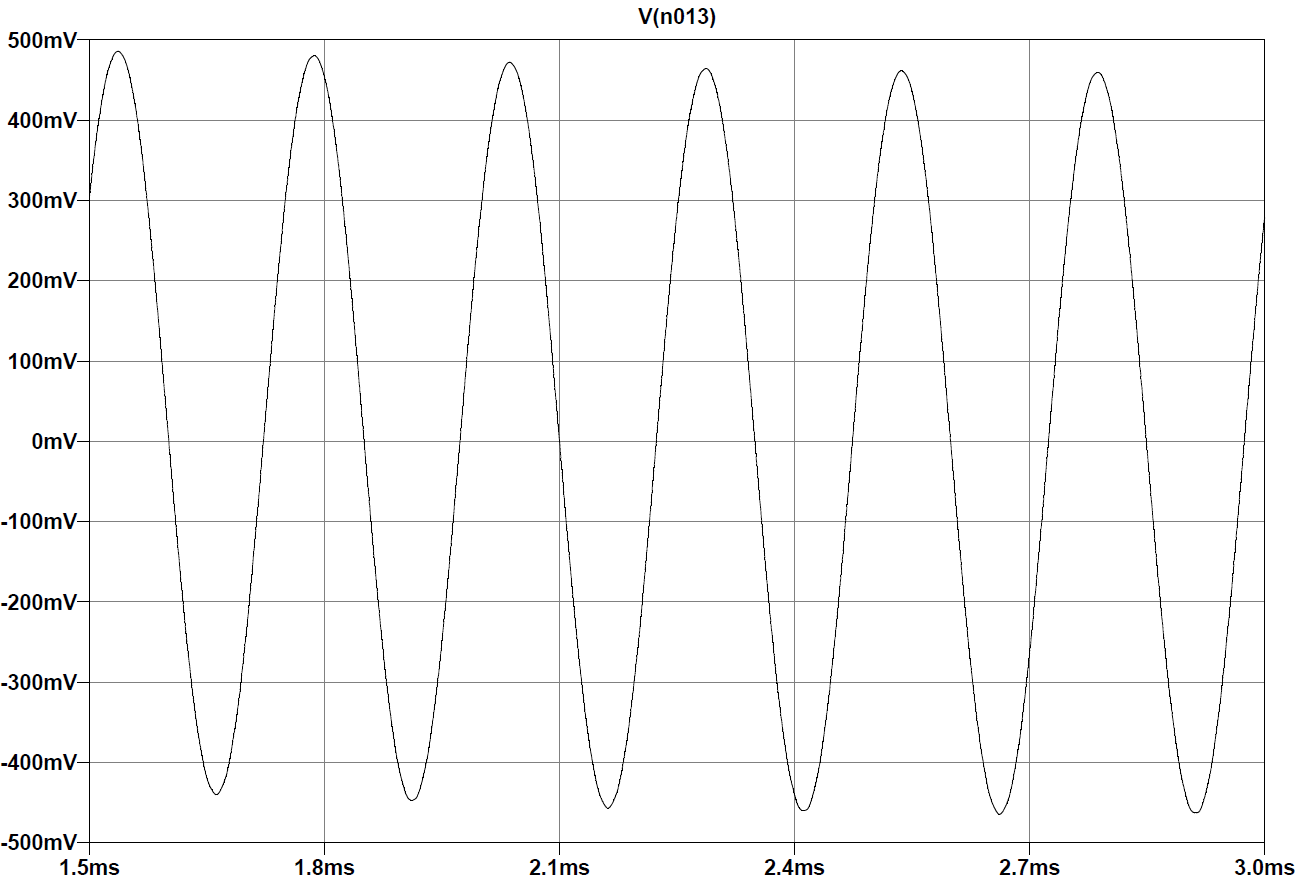
\includegraphics[width=\linewidth]{bpf/bpf4k}
			\caption{}
			\label{fig:bpf4k}
		\end{subfigure}
		
		\caption{Output of bandpass filter for message signals of (a) \SI{500}{\Hz}, (b) \SI{4}{\kHz}.}
		\label{fig:bpfout}
	\end{figure}

	\clearpage %%%%%%%%%%%%%%%%%%%%%%%%%%%%%%%%%%%%%%%%%%%%%%%%%%%	
	\subsection{Schmitt Trigger}
	From the output of the bandpass filter, the message signal will be recovered as a sine wave. From this wave, a Schmitt trigger will be used to convert the sinusoid to a square wave, effectively as a comparator. This is accomplished by pulling an op-amp to saturation using the non-inverting input of the op-amp. The minimum voltages required to trigger the jump from each saturation voltage is determined by the resistances, \begin{align*}
		V_{I\pm} & = -\frac{R_1}{R_2} \left( \mp V_{sat}\right)
	\end{align*}
	
	\begin{figure}[h]
		\centering
		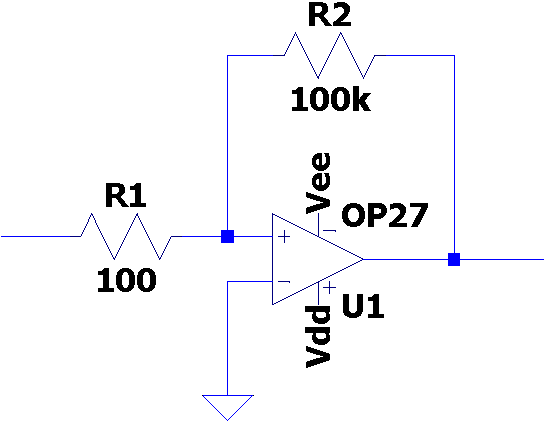
\includegraphics[width=0.3\linewidth]{schmitt/schmittckt-crop}
		\caption{The Schmitt trigger circuit as used in the circuit.}
		\label{fig:schmittckt-crop}
	\end{figure}

	In this circuit, a low threshold will be used in the Schmitt trigger by choosing \begin{align*}
		R_1 & = \SI{100}{\ohm} \\
		R_2 & = \SI{100}{\kohm}
	\end{align*}
	From this, when the input wave cross a threshold of \SI{11}{\mV}, the Schmitt will pull the voltage to the corresponding positive or negative saturation voltage.
	\subsubsection{Simulation}
	This trigger was simulated for both frequencies in the time-domain, as shown in Figure \ref{fig:schmittimg}.

	\begin{figure}[h]
		\centering
		\begin{subfigure}{0.9\linewidth}
			\centering
			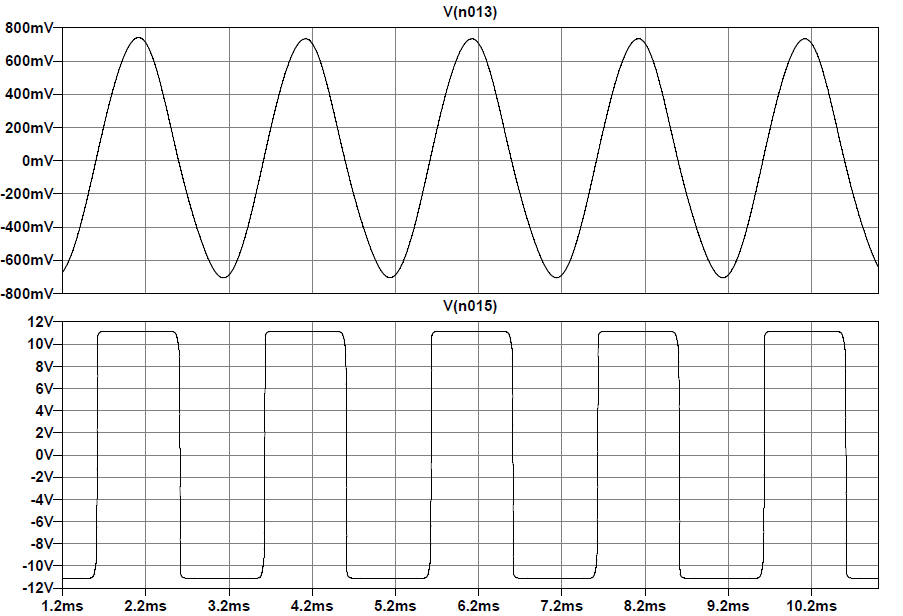
\includegraphics[width=\linewidth]{schmitt/schmitt500img}
			\caption{}
			\label{fig:schmitt500img}
		\end{subfigure}
		
		\begin{subfigure}{0.9\linewidth}
			\centering
			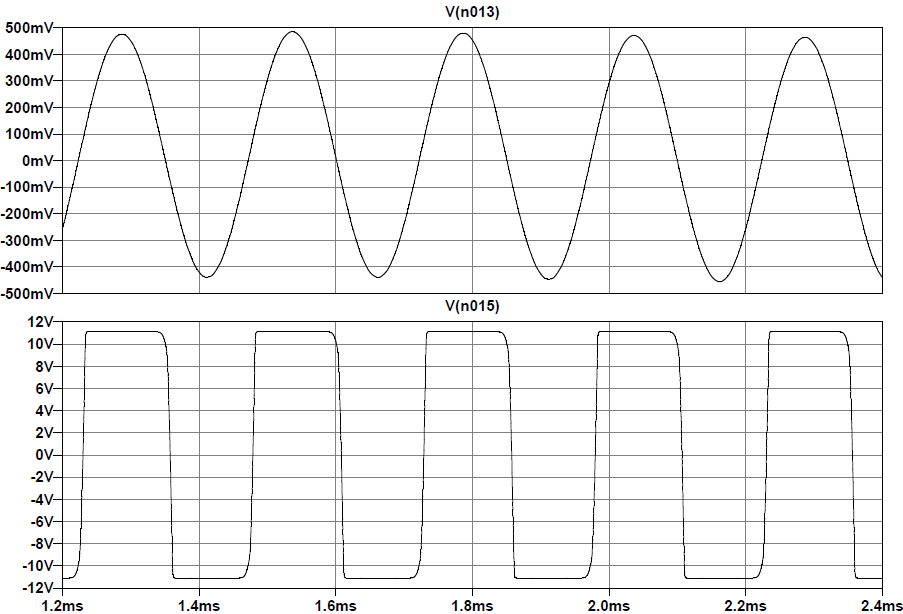
\includegraphics[width=\linewidth]{schmitt/schmitt4000img}
			\caption{}
			\label{fig:schmitt4000img}
		\end{subfigure}
		
		\caption{Output of Schmitt trigger for message signals of (a) \SI{500}{\Hz}, (b) \SI{4}{\kHz}.}
		\label{fig:schmittimg}
	\end{figure}

	\clearpage %%%%%%%%%%%%%%%%%%%%%%%%%%%%%%%%%%%%%%%%%%%%%%%%%%%
	\subsection{Buffer Amplifier}
	Lastly, a half-wave rectifier and a simple buffer amplifier is used to drive a speaker. Here, a MOSFET is used as a switch to drive a low-impedance speaker. A voltage divider is used to adjust the gate voltage relative to the square-wave signal input--in turn adjusting the amplitude of the output sound waves. The figure for this is shown in Figure \ref{fig:speakerckt-crop}. In the circuit, the volume is adjusted to $66\%$ of the magnitude of the input waveform.
	
	\begin{figure}[h]
		\centering
		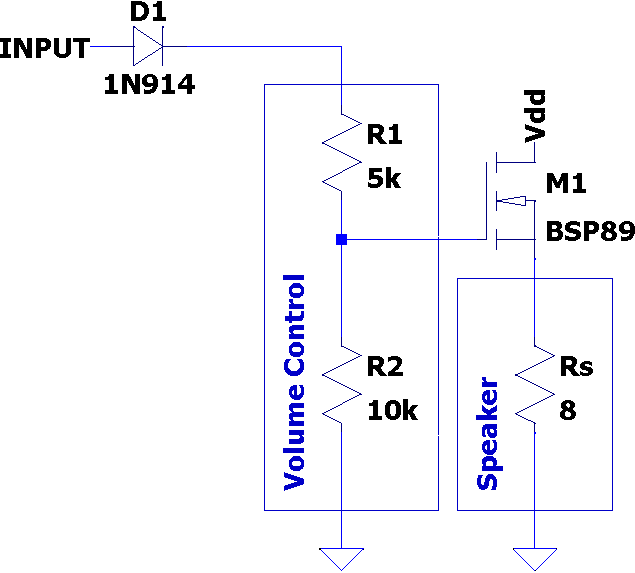
\includegraphics[width=0.5\linewidth]{speaker/speakerckt-crop}
		\caption{The buffer amplifier and driver for the \SI{8}{\ohm} speaker.}
		\label{fig:speakerckt-crop}
	\end{figure}
	
	
	\subsubsection{Simulation}
	At both frequencies, the amplifier was simulated in the time domain, as shown in Figure \ref{fig:speakerout}. At this current resistor configuration, the peak voltage seen by the speaker is \SI{3.7}{\V}.
	
	\begin{figure}[h]
		\centering
		\begin{subfigure}{0.9\linewidth}
			\centering
			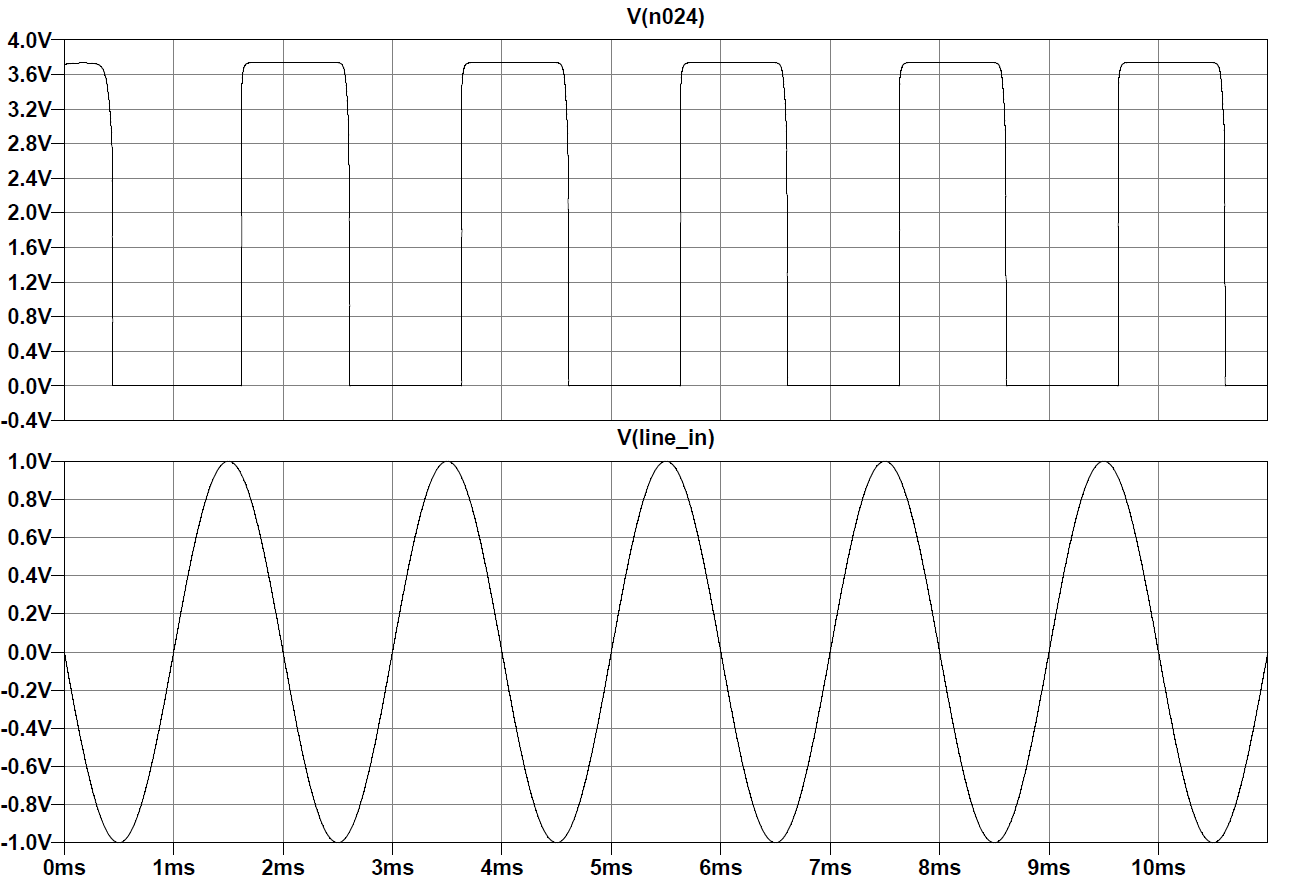
\includegraphics[width=\linewidth]{speaker/speaker500img}
			\caption{}
			\label{fig:speaker500img}
		\end{subfigure}
		
		\begin{subfigure}{0.9\linewidth}
			\centering
			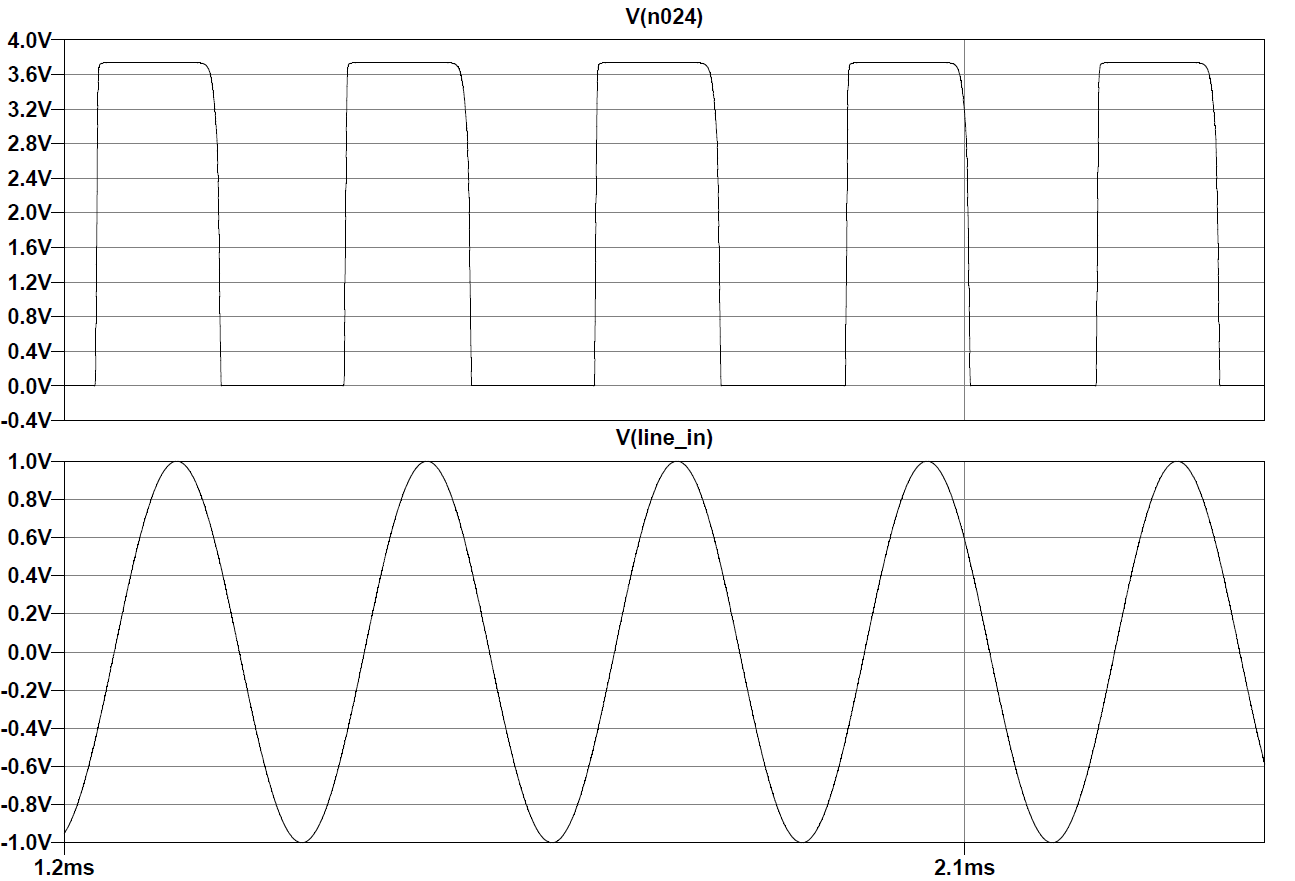
\includegraphics[width=\linewidth]{speaker/speaker4kimg}
			\caption{}
			\label{fig:speaker4kimg}
		\end{subfigure}
		
		\caption{Output of buffer amplifier driving the speaker.}
		\label{fig:speakerout}
	\end{figure}

	
	\clearpage %%%%%%%%%%%%%%%%%%%%%%%%%%%%%%%%%%%%%%%%%%%%%%%%%%%	
	\section{Conclusion and Discussion}
	An AM transmitter and receiver was designed and simulated using LTspice. The designed met the required specifications and the outcome of the project was successful. Overall, the design can use several improvements to make the transmission more robust in the real-world. Although the project was simulated, it would be expected to work on a physical system with not many adjustments.
	
	It should be noted that the design has several major drawbacks that could be fixed in iterative versions. First, the carrier oscillator is bound to drift significantly with time as both the resistances and capacitances of are bound to change with temperature. Additionally, there is no feedback in place aside from the RC-network gain. A recommendation would be to implement a crystal oscillator or to use a PLL attached to an external signal source.
	
	Next, both the bandwidth and amplitude of the transmitter and receiver is bound by the limitations of amplitude modulation. Other methods of transmitting signals offer more-robust methods at the cost of higher complexity. One major flaw of this project was the simulation and whether or not LTspice accurately depicts real-world components. It is likely that building this circuit on a breadboard would lead to additional trimming and perhaps a redesign of some components.

	\bibliographystyle{unsrt}
	\bibliography{final_report_bib}
	
	\clearpage
	\subsection*{Appendix A}
\noindent\begin{lstlisting}[language=matlab, caption={\noindent MATLAB code for iterating over component values for the high-Q bandpass filter.},label={lst:highqbpf}]
F_0 = 74000;              % (carrier) frequency of the oscillator
W_0 = 2*pi*F_0;           % Hz to rad/s
B   = 2*(2 * pi * 4000);  % bandwidth = 8 kHz
C   = 1e-9;               % choosing a common cap
%%%%%%%%%%%%%%%%%%%%%%%%%%%
%R3 = 2/(B * C);          % to get a perfect value for R3
R3 = 40000;               % ~40k
%R1 = 1/(B * C);          % similarily for R1
R1 = 20000;               %
%%%%%%%%%%%%%%%%%%%%%%%%%%% 
%R2 = 100 + 10 + 4.7;     %
R2 = 100;                 %

Req    = 1/(1/R1 + 1/R2);
W_test = sqrt(1 /(Req * R3 * C*C));
F_test = W_test / (2*pi);
\end{lstlisting}

	\begin{figure}[h]
		\centering
		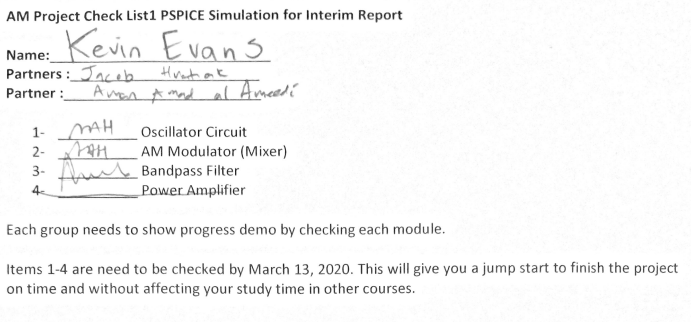
\includegraphics[width=\linewidth]{signoff}
		\caption{Sign-off sheet for the interim report.}
		\label{fig:signoff}
	\end{figure}
	
\end{document}